\documentclass[12pt,preprint]{aastex}

%\documentclass[iop,apjl]{emulateapj}
\usepackage{amsmath}
%\bibliographystyle{hapj}


\usepackage{graphicx}
\usepackage{natbib}
%\usepackage{colortbl}
\newcommand{\vdag}{(v)^\dagger}
\newcommand{\myemail}{m.morscher@u.northwestern.edu}
%\usepackage{subfigure}
\usepackage{epsfig}
%\usepackage{subfig}
%\usepackage{multirow}
%\usepackage{array}

\usepackage{caption}
\usepackage{subcaption}
%\renewcommand{\topfraction}{0.85}
%\renewcommand{\textfraction}{0.1}
\usepackage{changepage}

%\shorttitle{Black Holes in Star Clusters}
%\shortauthors{Morscher et al.}




\begin{document}

\title{Stellar-Mass Black Holes in Globular Clusters}
  
\author{Meagan Morscher, Carl Rodriquez, Stefan Umbreit, and Frederic A.\ Rasio}

\affil{Center for Interdisciplinary Exploration and Research in
  Astrophysics (CIERA), and Department of Physics and Astronomy,
  Northwestern University, 2145 Sheridan Road, Evanston, IL 60208,
  USA.}

\email{m.morscher@u.northwestern.edu}
\email{s-umbreit@northwestern.edu}
\email{rasio@northwestern.edu}



\begin{abstract}
We investigate the dynamical evolution of globular clusters containing a large number of stellar-mass BHs. Our main goal is to see whether it is possible for clusters to retain a significant number of BHs for $\sim 10\,$ Gyr and still resemble the Milky Way's population of old globular clusters (GCs). We use a Monte Carlo method, which allows us to model large-$N$ clusters with all the relevant physics required to describe these systems accurately. We present a grid of 42 realistic Monte Carlo simulations that span a range of initial physical properties. We find that under standard assumptions for initial cluster models, including the initial BH population, many of our models that survive to $\sim 10\,$ Gyr still contain a significant number ($\sim 100-1000$) of BHs at the end of the simulation. This population of retained BHs produces a heating effect which prevents the cores of most of our models from collapsing down to the sub-parsec scale that is typical for MW GCs. However some of our models have observable properties similar to real GCs....(\textbf{state which ones}). 

Our results suggest the need to revisit our understanding of BH formation and observational studies of BHs, including the BH mass function as well as the strength of supernova kicks for BHs.
	% ABSTRACT STILL NEEDS SOME WORK

\end{abstract}



%%%%%%%%%%%%%%%%%%%%%%%%%%%%%%%%%%%%%%%%%%%%
%%%%%%%%%%%%%%%%                                             %%%%%%%%%%%%%%%%
%%%%%%%%%%%%%%%%      INTRODUCTION        %%%%%%%%%%%%%%%%
%%%%%%%%%%%%%%%%                                             %%%%%%%%%%%%%%%%
%%%%%%%%%%%%%%%%%%%%%%%%%%%%%%%%%%%%%%%%%%%%

\section{Introduction} \label{Intro}

Massive star clusters should form $\sim 100\, -\, 1000$ stellar-mass black holes (BHs) 
through normal stellar evolution, and as long as BH birth kicks are sufficiently low, most
should be retained in the cluster initially. Through dynamics, these BHs will become 
members of binary systems with either 
stellar or dark remnant companions, and evolve to produce X-ray binaries (XRBs) or 
merging compact object binaries, which will be detectable by future gravitational wave 
(GW) observatories (e.g. LIGO; \citealt{HarryLIGO2010}). These systems can, in theory, 
be found either inside of clusters or in the field. It is well known that the formation rate 
per unit mass of XRBs is orders of magnitude larger in clusters than it is in the field
(e.g., \citealt{Pooley2003}), which suggests that stellar dynamics must play an essential
role in producing XRBs in present day clusters. Since the early nineties, however,  
theoretical arguments, simulations and observations have all suggested that old GCs 
should have very few ($\sim1$) BHs at present. Early studies (\citealt{Kulkarni1993}, 
\citealt{Sigurdsson1993}) predicted from analytic arguments that the BHs, being heavier
than other stars, should rapidly segregate to the cluster center through dynamical friction
against the lighter background stars and eventually succumb to the so-called Spitzer
instability \citep{Spitzer1969, Kulkarni1993}. If this happens, the BHs will form a dense 
subsystem within the cluster core that consists primarily of BHs, and is dynamically 
decoupled from the cluster. The small-$N$ sub-cluster of BHs has a very short relaxation 
time, so it will undergo its own core collapse, begin to form hard binaries through three-body 
interactions, and subsequently begin ejecting single and binary BHs. The system of BHs 
will evaporate within a few Gyr, leaving behind a cluster essentially devoid of 
BHs. Other theoretical studies confirmed this idea through idealized simulations 
(e.g., \citealt{PortegiesZwart2000}, \citealt{OLeary2006}). Over the last several years, 
however, our understanding about BHs in dense star clusters has shifted quite dramatically.

The old story began to change when the first BH X-ray binary was detected inside of an 
old GC in an external galaxy, NGC 4472 \citep{MaccaroneNature2007}. Several more BH 
XRBs were subsequently discovered inside of GCs (\citealt{Barnard2011}, \citealt{Shih2010}). 
Recently, \cite{Strader2012} discovered \emph{two} BHs inside of the Milky Way GC M22. 
These BHs are the first ever to be found in a GC in our \emph{own} galaxy, as well as the first 
to be \emph{discovered} through radio observations. By assuming that these systems are 
BH-WD binaries, they used published theoretical calculations from \cite{Ivanova2010} to 
estimate the fraction of present-day BHs in GCs that are actively accreting from a WD 
companion. They estimate that the detection of two accreting BHs in M22 implies a true 
population of $\sim 5-100$ BHs.  The same group recently found another BH in a different 
galactic GC, M62, also through radio observations \citep{Chomiuk2013}. 

On the theoretical side, a few recent studies have provided hints that old clusters might be able to retain BHs for many Gyr. \cite{Mackey2008} used $N$-body simulations of clusters with BHs to explain the radius-age trend in the Magellanic Cloud clusters. With models of varying initial BH retention, they found that a population of retained BHs could provide a heat source for some clusters, providing a possible explanation for the observed spread in the radii of Magellanic Cloud clusters. In some of these models, significant numbers of BHs (as many as $\approx 100$) were retained for $\sim$ 10 Gyr. 
%\cite{Moody2009} use semi-analytic calculations of the dynamics of BH-binary interactions in clusters to study the rate of BH mergers. They find that in their most massive and metal-rich clusters, 5\% of their BH-binaries are actually retained.
\cite{Sippel2013} present a scaled-down (in mass) direct $N$-body model of M22, known to host \emph{two} stellar-mass BHs. At an age of 12 Gyr, their model retains 16 BHs (about 1/3 of the initially-retained population), which is consistent with the prediction of \cite{Strader2012}. A Monte Carlo study by \cite{Morscher2013} found that some clusters may retain as many as \emph{hundreds} of BHs for 12 Gyrs.  The long-term survival of such a large number of BHs is explained by the fact that the BHs do not become Spitzer unstable on the whole, but rather the majority of BHs remain well mixed with the rest of the cluster throughout the entire 12 Gyr evolution.

A very different study by \cite{Breen2013} focused on the evolution of two-component clusters, with a population of BHs co-existing within a cluster of light stars. They provide theoretical calculations as well as direct $N$-body simulations which both suggest that the flow of energy in the system is ultimately determined by the cluster. In this way, the rate of energy production in the BH subsystem as well as its evaporation rate is regulated by the cluster as a whole. This implies that BHs can survive for much longer than previously thought (i.e., for $\sim 10\, T_{rh,i}$, where $T_{rh,i}$ is the initial half-mass relaxation timescale) because their dynamical evolution happens on the relaxation timescale of the \emph{cluster}, rather than that of the BH subsystem. This result suggests that the long-standing belief that BHs will dynamically decouple from clusters may be incorrect, which would imply that the foundation for the argument that old clusters should be deplete of BHs does not hold up.

The topic of BHs in clusters is still worthy of further discussion. While the theoretical arguments presented in \cite{Breen2013} are interesting, these two-component models cannot be directly compared to real GCs, which have a  broad spectrum of stellar and BH masses, as well as larger total cluster masses. Several more-realistic studies have now predicted the survival of at least some BHs (e.g., \citealt{Mackey2008, Morscher2013, Sippel2013}), but there is still no definitive answer as to \emph{how many} might actually be hiding in old GCs at present. 
In this paper, we present a large grid Monte Carlo simulations of realistic, large-$N$, Milky-Way-like cluster and address the question of retention of BHs and structural evolution of clusters with BHs.
%There is still no large grid of realistic, large-$N$, Milky-Way-like cluster models that have addressed the question of retention of BHs and structural evolution of clusters with BHs. In the present paper, we address this need with a set of realistic Monte Carlo GC simulations. 
The rest of the paper is organized as follows:  FILL IN!


%%%%%%%%%%%%%%%%%%%%%%%%%%%%%%%%%%%%%%%%%%%%
%%%%%%%%%%%%%%%%                                             %%%%%%%%%%%%%%%%
%%%%%%%%%%%%%%%%       MONTE   CARLO       %%%%%%%%%%%%%%%%
%%%%%%%%%%%%%%%%               METHOD             %%%%%%%%%%%%%%%%
%%%%%%%%%%%%%%%%                                             %%%%%%%%%%%%%%%%
%%%%%%%%%%%%%%%%%%%%%%%%%%%%%%%%%%%%%%%%%%%%


\section{Monte Carlo Method}
\subsection{Overview of Method}
We use a Monte Carlo (MC) method for modeling the dynamical evolution of GCs.
While the direct $N$-body method is more exact than MC schemes, 
it can only simulate clusters with up to $N \sim 10 \times 10^5$ due to the
poor scaling with $N$ (computation time $\sim N^3$). In order to model large MW GCs
with initial $N$ up to $\sim 10^6$, we must employ a Monte Carlo (MC) technique. 
\emph{SHOULD I CUT ITALICIZED SECTION? In contrast to the direct $N$-body method, 
which directly integrates the equations 
of motion of all particles, the MC method, cluster evolution is approximated using the 
theory of two-body relaxation. Stellar orbits are not resolved on a dynamical
timescale. Instead, the constants of motion for each star, energy $E$ and angular 
momentum $J$, are stored. On the relaxation timescale, many long-range,
weak gravitational scattering interactions among stars perturbs the stellar orbits, 
 leading to a flow of energy from the cluster core outwards, and driving 
 cluster evolution. In the MC method, this is treated with a single interaction
  among each pair of stars per time step, where this single effective interaction 
  represents the cumulative effect of many gravitational interactions over
   the time step.} In MC methods, computation time scales as 
   $\sim N$ log$N$, which makes it feasible to model large
 GCs and to study the evolution of rare objects, such as BHs.

Our MC implementation is a variation of the ``orbit-averaged Monte Carlo 
method" developed by \cite{Henon1971a} for solving the Fokker-Planck 
equation. The details of our method are described in \citealt{Joshi2000}, 
\citealt{Joshi2001}, \citealt{Fregeau2003}, \citealt{Fregeau2007} and 
\citealt{Chatterjee2010}. Here we highlight the most important details for
the present study. We treat the cluster on a star-by-star basis, and so we
can easily add complexity, such as stellar evolution and strong binary 
interactions. Stars and binaries are evolved according to the stellar
evolution fitting formulae and interacting binary evolution calculations
of SSE and BSE (\citealt{Hurley2000}, \citealt{Hurley2002}). We use a 
the modified stellar remnant formation prescription of \cite{Belczynski2002}, 
which produces BH masses in the range $\sim 5-30\, M_\odot$ for $Z=0.001$. 
Both neutron stars (NS) and BHs receive natal kicks
assumed to be generated by the asymmetric ejection of mass during 
a supernova explosion. NS kicks are drawn from a Maxwellian
distribution with $\sigma$=265 km s$^{-1}$. BHs are expected to receive
much lower velocity kicks (see \citealt{Wong2012} and references therein),
and thus we follow the prescription of \cite{Belczynski2002} to reduce the
kick magnitude according to the amount of material that falls back onto the 
final BH after the supernova explosion, based on the theoretical calculations of 
\cite{Fryer2001}.  In this prescription, BHs that form via direct collapse 
 (i.e. all material falls back onto the BH) do not receive natal kicks.
BSE calculates the orbital evolution due to emission of GW radiation in compact
 object binaries, which is important for tracking the mergers of 
BH-BH binaries. Once a binary is ejected from the cluster, however, 
it is no longer evolved with our MC code.
For these systems, we estimate the merger time using a simplified timescale 
for GW in spiral in the weak field limit \citep{Peters1964} based on the system's
properties at the time of ejection.

In addition to two-body relaxation, we account for
strong binary interactions between either a binary and a single star (BS)
or two binaries (BB). Strong interactions are chosen using MC sampling
based on the cross-section for a close interaction between the pair of 
neighboring objects, and these interactions are then integrated 
directly using FEWBODY. These resonant binary interactions allow for many
important effects within binary systems, such as exchanges, binary hardening,
ionization, and ejections, all of which are relevant for the evolution of BHs in clusters.


%%%%%%%%%%%%%%%%%%%%%%%%%%%%%%%%%%%%%%%%%%%%
%%%%%%%%%%%%%%%%                                             %%%%%%%%%%%%%%%%
%%%%%%%%%%%%%%%%                  3BB                   %%%%%%%%%%%%%%%%
%%%%%%%%%%%%%%%%          FORMATION           %%%%%%%%%%%%%%%%
%%%%%%%%%%%%%%%%                                             %%%%%%%%%%%%%%%%
%%%%%%%%%%%%%%%%%%%%%%%%%%%%%%%%%%%%%%%%%%%%



\subsection{New Physics: Three-body Binary Formation}

We have recently implemented a simplified prescription for three-body 
binary formation, a process that is expected to produce an important 
population of hard BH-binaries 
\citep{Kulkarni1993, Sigurdsson1993, PortegiesZwart2000,OLeary2006,  
Banerjee2010}, and is therefore extremely important for this study. 
If three single stars experience a close resonant encounter, it is possible for two
of the stars to become gravitationally bound to one another, with the third star 
carrying away the extra energy. The probability
of binary formation is usually quite low, and realistically only becomes possible 
under the extreme conditions expected at the core of a cluster which has been driven
to collapse by a population of BHs. We restrict our attention to 
dynamically hard binaries, as only hard binaries are expected to survive within the
cluster environment \citep{Heggie1975}.
Our simplified prescription relies on the calculation of the rate at which 
three neighboring single BHs will form a hard binary. Using the calculated rate
and the current timestep, we can estimate the probability that the three-body
 system will result in binary formation, and then use MC sampling to select which systems
  will actually form a new binary.

% This is copied from my ApJ letter...must rephrase
Our prescription is similar to that of 
\citet{Ivanova2005}, \citet{Ivanova2010}, and \citet{OLeary2006},
where the rate is expressed as a function of binary hardness,
which ratio of the binding energy of the binary to the average local stellar kinetic energy,
\begin{equation}
\eta = \frac{G \, m_1 \, m_2}{r_p \, \langle m \rangle \, \sigma^2}.
\label{eq:eta}
\end{equation}
Here $m_1$ and $m_2$ are the masses of the two stars assumed to
form a binary, $r_p$ is their separation at pericenter, and $<m>$  and $\sigma$ are
the local average mass and velocity dispersion.

Keeping both the geometric and gravitational focusing contributions to
the cross-section (in contrast to \citealt{Ivanova2010}, where the  % REPHRASE
geometric part of the cross section for the third star to interact
with stars 1 and 2 is dropped), we construct an expression for the
rate of binary formation for the selected neighboring three stars.
 For local number density, $n$, and
average relative velocity at infinity, $v_{\infty}$, the rate at which
two stars ($m_1$ and $m_2$) form a binary with hardness $\eta \, \geq
\, \eta_{\rm min}$ through an interaction with a third star ($m_3$) is
given by
\begin{multline}
\Gamma(\eta \geq \eta_{min}) = \sqrt{2} \pi^2 n^2
      {v_{\infty}^{-9}} \\ \times (m_1 + m_2)^5 \eta_{\rm min}^{-5.5} (1 + 2
      \eta_{\rm min}) \\ \times \left[ 1+2 \eta_{\rm min} \left( \frac{ m_1 + m_2 +
            m_3}{m_1 + m_2 } \right) \right].
\label{eq:Gamma}
\end{multline}
This requires the calculation of the local $n$ and $v_{\infty}$ using a subset
of nearby stars (see next section for details).
When a binary is formed, we choose a
value for $\eta$ from a distribution according to the differential
rate, d$\Gamma$/d$\eta$, with lower limit $\eta_{\rm min}$. 
Assuming conservation of momentum and energy, the rest of the 
properties of the new system can be calculated. 

Binaries that are too soft are likely to be destroyed rather quickly,
whereas tight binaries with binding energy at least as large as the 
local kinetic energy of stars can remain intact through binary interactions
 \citep{Heggie1975}. We therefore restrict our attention to locally
 hard binaries by requiring that newly formed binaries have
$\eta \geq 5 = \eta_{\rm min}$, which also factors into the calculated rate.
When forming a three-body binary, we choose a
value for $\eta$ from a distribution according to the differential
rate, d$\Gamma$/d$\eta$, with lower limit $\eta_{\rm min}$. The rest
of the properties of the system are calculated from conservation of
momentum and energy.
We allow only BHs to form binaries, since they 
are most likely to be found near the cluster center where the density is large 
enough for binary formation to occur. 
% End section copied from ApJ letter

\section{Comparison with $N$-Body}


The Monte Carlo approach requires the calculation of the local average of several
physical quantities.  For example, the physics of three-body binary formation and the
selection of the relaxation time both depend upon
local averages of the number density, velocity dispersion, and average mass of
the cluster at a specific radius \citep{Joshi2000}.
However, it is not the case that these averages should be computed over the same
number of stars.   While three-body binary formation should depend only on the
properties of the closest stars, the relaxation time step must be applied broadly to
 the entire cluster, and therefore should be selected to be appropriate for the entire cluster.
 We both expect and require three-body binary
formation to be more sensitive to local spikes in number density and velocity
dispersion than the cluster-wise relaxation time.  Therefore, we must adjust the
number of stars over which to compute an average depending on the scale of the
physics in question.

\begin{figure}[h!]
  \includegraphics[scale=0.65]{64.pdf}
  \caption{Evolution of 2-Species Plummer models as computed by the Monte Carlo
  approach and the direct N-body approach of \cite{Breen2013}.  The
  top plot shows the half-mass radius (on top) and core radius (bottom) for the
  two methods, while the lower plot shows the number of retained black holes as
  a function of time.}
  \label{fig:2species64k}
\end{figure}


As in previous studies \citep{Joshi2000} we determine the optimal code
parameters by direct comparison to $N$-body simulations with identical initial
conditions.  Since the primary focus of this study is the retention of black holes,
we choose as our comparison an idealized two-component model recently studied 
in \cite{Breen2013} which provides a simplified description of the evolution of a population
of stellar-mass BHs in a cluster. These models are a realization of standard Plummer
sphere populated by a large population of low-mass stellar objects and a smaller
population of heavy objects.  We consider models with an individual mass ratio of
$m_2/m_1 = 20$, and a total cluster mass ratio of $M_2/M_1 = 0.02$, where $m_1$
and $m_2$ are the masses of individual particles, and $M_1$ and $M_2$ are the
total masses of each component.  We performed comparison simulations with $64k$ 
and $128k$ particles, although only the $64k$ runs are illustrated here.

In Fig. \ref{fig:2species64k}, we compare the cluster properties as reported by
the $N$-body simulations of \cite{Breen2013} to the results of our Monte
Carlo technique.  Empirically, we find optimal agreement by computing the
average quantities over the nearest 40 stars for two-body relaxation, and the
nearest 6 stars for three-body binary formation.  In particular, the 
evaporation rate of the black-hole subcluster in our simulations replicates
the $N$-body results extraordinarily well up to the ejection of the final
black-hole binary from the cluster.  Furthermore, we find the Monte Carlo
approach correctly reproduces the time evolution of the half-mass radius
to within 8\% after $2\times10^5$ $N$-body time units.  

Of the measured cluster properties, only the core radius cannot be
reproduced correctly by the Monte Carlo approach.  Immediately following core
collapse, the measured core radius for the Monte Carlo differs from the $N$-body
results by as much as 65\%.  Unfortunately this is to be expected: once mass
segregation and core collapse have occurred, the cluster core is comprised almost
entirely of black holes which have dynamically decoupled from the rest of the
cluster.  Correctly modeling the internal dynamics of an $N\sim100$ system using
a MC approach has very little hope of success; however, as the black holes are
ejected, and the core becomes populated with a larger number of lighter halo
stars, the validity of the MC approach is restored, and the core
radius better resembles that of the N-body approach.  Additionally, the core radius
is known to very sensitive to physical effects, such as three-body binary formation,
which is a stochastic process. New techniques are under
investigation that will correctly evolve the subcluster dynamics while
maintaining the speed of the MC approach. \textbf{For the present study,
we are encouraged by previous results from \cite{Morscher2013} suggesting
 that the BHs might actually never decouple from the cluster on the whole, 
 in which case a MC approach is appropriate.}



%%%%%%%%%%%%%%%%%%%%%%%%%%%%%%%%%%%%%%%%%%%%
%%%%%%%%%%%%%%%%                                             %%%%%%%%%%%%%%%%
%%%%%%%%%%%%%%%%                 INITIAL              %%%%%%%%%%%%%%%%
%%%%%%%%%%%%%%%%          CONDITIONS          %%%%%%%%%%%%%%%%
%%%%%%%%%%%%%%%%                                             %%%%%%%%%%%%%%%%
%%%%%%%%%%%%%%%%%%%%%%%%%%%%%%%%%%%%%%%%%%%%



\section{Initial Conditions}

We have calculated the dynamical evolution of 42 cluster models with a wide range of
initial conditions. All models are initialized as King models and with stellar masses 
drawn from the \cite{Kroupa2001} initial mass function (IMF) from 
0.1 \,-\, 100$\, M_\odot$. We vary the initial number of stars 
($N=2 \times 10^5$, $8 \times 10^5$, and $1.6 \times 10^6$), the initial King 
concentration parameter ($W_o=2$, 5, 7) and the Galactocentric distance $R_G$, 
which in our models corresponds to three different metallicities
($Z=0.005$ at $R_G=2$ kpc, $Z = 0.001$ at $R_G\,=\,8$ kpc and $Z=0.0001$ at $R_G=20$ kpc). 
These initial conditions form a $3 \times 3 \times 3$ grid of 27 cluster models. 
Each of these models has initial virial radius $r_v\,=\,2$ pc and binary fraction
 $f_b = 10$\%. The choice to vary metallicity as a function of $R_G$ was 
 motivated by the currently observed properties of the Milky Way's GC population, 
 which show a correlation between $R_G$ and $Z$, with larger metallicities 
 corresponding to being found closer to the Galactic center \textbf{(ADD REF)}.

Beyond the $3 \times 3 \times 3$ grid, we have run fifteen additional models
in which we have either varied a new parameter, or extended the range of one of the 
parameters from our $3\times3\times3$ sweep. For each $N$, starting with our 
intermediate parameters ($W_o$ = 5, $R_G$=8 kpc, $Z$=0.001),
we created models with larger central concentration ($W_o$ = 11), with smaller and
larger initial binary fraction ($f_b$ = 1\% and 50\%), and smaller and larger virial radius 
($r_v$ = 1 and 4 pc). We do not attempt to reproduce the distribution of GCs with 
different properties, but rather our goal is to see whether GCs with many BHs can 
evolve into $\sim 10\, \rm Gyr$ old clusters that are consistent with the properties of MW GCs. 
We evolve all of our models to 12 Gyr\footnote{Three of our low-$N$ models evaporated
before 12 Gyr, ending the simulation early}, which is a typical age for MW GCs. 
The properties of our initial models are give in Table \ref{table:initial_conditions}.


%\subsection{Initial Black Hole Populations}
For typical IMFs (e.g., Kroupa, Salpeter), a fraction of $\sim 10^{-4}\, - \,10^{-3} \, N$ 
stars will become BHs. For our low-, intermediate- and large-$N$ models, 
we form $\approx 450$, 1750, and 3500 BHs, respectively. The initial BH mass spectrum
is shown for a subset of models in Figure \ref{fig:BHmasses}. 









%%%%%%%%%%%%%%%%%%%%%%%%%%%%%%%%%%%%%%%%%%%%
%%%%%%%%%%%%%%%%                                             %%%%%%%%%%%%%%%%
%%%%%%%%%%%%%%%%              RESULTS            %%%%%%%%%%%%%%%%
%%%%%%%%%%%%%%%%                                             %%%%%%%%%%%%%%%%
%%%%%%%%%%%%%%%%%%%%%%%%%%%%%%%%%%%%%%%%%%%%


\section{Results of Simulations}

\subsection{Description of Overall Evolution}

We now describe the overall evolution common to all of our models. The BHs form
within about 10 Myr and with masses $\sim 10$ times that that of typical stars, 
the BHs begin to sink due to dynamical friction against the light background stars. 
The timescale for segregation of the BHs from about the the half mass radius to the core is 
\begin{equation}
t_{seg} \sim \frac{\langle m \rangle}{M_{BH}} t_{rh}
\label{eq:segregation timescale}
\end{equation}
where $\langle m \rangle$ is the average stellar mass, $M_{BH}$ is the mass of the BHs, 
and $t_{rh} \sim$ a Gyr is the half mass relaxation time. Since this timescale is dependent
on the BH mass, the heaviest BHs tend to sink to the core the fastest, driving a central collapse
(note: this is different from what is referred to as \emph{core collapse}, which occurs on a much longer
timescale). This can be seen in Figure \ref{fig:LagRad}, which shows the lagrange radii
for a subset of our models. We plot the lagrange radii separately for the BHs (solid lines) 
and for the non-BHs (dotted lines), which shows a clear separation of these two populations
over time, with the BHs being more centrally concentrated than lighter stars. 
Note that only a small subset of the BHs sink \emph{deeply}, while most of the 
BHs remaining well mixed with the rest of the cluster. The collapse of the innermost BHs 
allows the core to reach high enough density that hard BH--BH binaries can be formed
via three-body interactions. In this high density environment, these binaries, 
and potentially primordial binaries as well, experience strong binary interactions 
which can eject objects from the core or from the cluster entirely, injecting heat
into the cluster and causing the core oscillations seen in Figure \ref{fig:LagRad}.

In Figure \ref{fig:bhs_vs_time} we show the total number of BHs retained within 
each cluster model as a function of time. The initial increase in number of BHs within
$\approx 10$ Myr shows the period of BH formation. Soon after the BHs have segregated,
the number of retained BHs begins to decrease as BHs are dynamically ejected, and 
this continues through the end of the simulation. Since density increases with $N$, the 
larger-$N$ models have higher rates of BH ejection, consistent with the higher rate
of strong binary encounters. Despite the larger interaction rate, the fraction of initially 
retained BHs that survive within the cluster models for 12 Gyr is smallest for the lowest $N$
models ($f_{ret,final} \approx 20$\%) and largest for the high $N$ models ($f_{ret,final}
\approx 50$\%). This reflects the fact that the lower $N$ models are more dynamically 
evolved than their large-$N$ counterparts after the same amount of physical time, since
their relaxation time is shorter for the lower-$N$ models. 
The majority of our low-, intermediate-, and high-$N$ models end with $\approx 50-100$ BHs,
$\approx 400-800$ BHs, and $\approx 1000-2000$ BHs, respectively, but the total range of
retained BHs spans from $9-1988$. Most of these BHs are single objects.


In Figure \ref{fig:CumBinintEscBHs} we show the cumulative number of binary-binary
(B-B) and binary-single (B-S) interactions along with the total number of ejected single BHs, 
BH-BH binaries, and BH-other binaries, as a function of time. The early phase of rapid 
BH ejection represents BHs that are ejected at birth via supernova kicks prior to 10 Myr, 
and is followed by a flattening of the BH ejection rate, during which time the BHs
are segregating. By around 100 Myr, the binary 
interaction rate increases abruptly, and with it comes an increase in the BH ejection 
rate. In particular, the BH-BH ejection rate seems to be most sensitive to the B-B 
interaction rate. This is to be expected, since in a B-S interaction, assuming three stars of
comparable mass, it would be much more likely for the \emph{single} star to be 
ejected that the \emph{binary}. The binaries that have become tight enough to be 
ejected through strong interactions most often BH-BH binaries, since these interactions 
should tend to replace any lighter non-BH binary companions with the heavier BHs in 
the process. This explains why most of the number of ejected BH-BH binaries typically
more than an order of magnitude larger than the number of ejected BH-binaries with a 
non-BH companion. 


Figure \ref{fig:mass_evolution} 
shows the evolution of total cluster mass for all 42 models, separated by $N$.  Within the first 
few Myr, there is a phase of rapid mass loss from stellar evolution. After the most massive 
stars have evolved, the rate of mass loss slows to a nearly steady rate and is due to both 
tidal stripping and stars becoming gravitationally unbound by obtaining a velocity above
the cluster escape velocity. Most of our models lose about half of their mass by 12 Gyr. 
It is well known that clusters lose significant amount of their mass over Gyr timescales, which
is why the smallest clusters have already evaporated, and also why we must initialize
our models with at least twice the mass we wish to have at the end of the simulation.
In fact, our three models with $N=2 \times 10^5$ and the smallest  $R_G$ (2 kpc)
evaporate due to the tidal effect of the galaxy within 6 Gyr (dotted lines in the upper
left panel of Figure \ref{fig:mass_evolution}). 

In general, we find that the final cluster mass directly proportional to $R_G$, as expected. However, the models
 with $R_G$ of either 8  or 20 kpc tend to lose mass at a similar rate. In addition to $R_G$, 
 the initial virial radius also affects the cluster mass loss significantly, especially for small $N$ models, 
 which have shorter relaxation times, and thus are dynamically older than larger $N$ models at 12 Gyr. 
 For example, in the model with $N=2 \times 10^5$ and $r_v=1$ pc loses more than 80\% of its
  mass by the end of the simulation.  


 %%%%%%%%%%%%%%%%%%%%%%%%%%%%%%%%%%%%%%%%%%%%
%%%%%%%%%%%%%%%%                                             %%%%%%%%%%%%%%%%
%%%%%%%%%%%%%%%%           ANALYSIS              %%%%%%%%%%%%%%%%
%%%%%%%%%%%%%%%%              OF   BHs               %%%%%%%%%%%%%%%%
%%%%%%%%%%%%%%%%                                             %%%%%%%%%%%%%%%%
%%%%%%%%%%%%%%%%%%%%%%%%%%%%%%%%%%%%%%%%%%%%

\subsection{Analysis of BH Populations}

The final distribution of BH masses for  a subset of models is shown in Figure \ref{fig:BHmasses}
along with the mass distribution soon after the BHs are formed. We find that the heaviest BHs
are ejected first, consistent with the fact that the heaviest BHs (at any given time) are most likely
to be in the dense core region where they can participate in binary interactions. Over time,
the maximum BH mass in the cluster is reduced from $\approx 25-30 M_\odot$ down to 
$\approx 15-20 M_\odot$. Thus, even at the 12 Gyr, many of our models still contain a
substantial population of 10$M_\odot$ BHs.

The overall populations of retained and ejected BHs for each model are shown in 
Table \ref{table:initial_conditions}. As mentioned previously, most of the retained BHs
remain as single stars throughout the cluster evolution, with at most
tens of BH-binaries (of any type), and often fewer than ten. Of these binaries, the number
of BHs in binaries with another BH is comparable to the number that have a stellar companion.
There are a handful of BH-WD binaries across the set of models, but there are no BH-NS
binaries. For models with 
large-$N$ and binary fractions of $f_b=50$\% 
have significantly more BHs in binaries than models with lower $f_b$. For example
in the $N= 1.6 \times 10^6$ model with $f_b$=50\%, the number of BH binaries (of any type)
can be from about 3-8 times larger than the other models with the same $N$ but 
lower binary fractions (depending on other parameters). This indicates that it is not 
only three-body binaries formed in the 
core that involve BHs, but rather, a larger population of binaries provides more 
opportunity for BHs to exchange into a binary system.

Systems with smaller initial virial radii tend to eject BHs at a higher rate due to
the increased density, and thus end with significantly fewer
BHs (yellow curves on right panels of Figure \ref{fig:bhs_vs_time}), and the opposite is true for 
models with larger initial virial 
radius (blue curves on the same panels). We find that the models with smaller $R_G$ retain fewer BHs
at 12 Gyr, but this is mostly a reflection of the fact that they were not able to retain as many BHs
initially due to their smaller tidal radii. Figure \ref{fig:RetBHsSingleBinary}
shows the distribution of single versus binary BHs within a subset of models. Across all 
simulations, the majority of BHs present in the cluster are \emph{single}, 










%%%%%%%%%%%%%%%%%%%%%%%%%%%%%%%%%%%%%%%%%%%%
%%%%%%%%%%%%%%%%                                             %%%%%%%%%%%%%%%%
%%%%%%%%%%%%%%%%           OBSERVABLE       %%%%%%%%%%%%%%%%
%%%%%%%%%%%%%%%%           PROPERTIES         %%%%%%%%%%%%%%%%                                      
%%%%%%%%%%%%%%%%                                             %%%%%%%%%%%%%%%%
%%%%%%%%%%%%%%%%%%%%%%%%%%%%%%%%%%%%%%%%%%%%


\section{Observable Properties}

We compare the properties of our models at 12 Gyr to the observed properties of the galactic GCs. All quantities are taken from the \cite{Harris1996} catalog (2010 edition), except for the total cluster mass, which is taken from \cite{Gnedin1997}. For our models, the total cluster mass is simply the sum of the masses of all cluster stars, including both luminous and also dark objects. We have calculated the core radius ($r_c$), half-mass radius ($r_h$) and central luminosity density ($\rho_l$) using only the luminous objects in an attempt to measure similar properties to the those that observers would measure. 

One key observable property of GCs is the core radius, which is a central region of a cluster over which the density and velocity dispersion are roughly constant. To compute the core radius, observers generally start by binning the stars radially and then constructing a surface brightness profile (SBP) \textbf{REF!}. The core radius is then found either by fitting a king model to the SBP, or by finding determining the radius at which the luminosity density drops to half the central value. The problem with this is that, since the stars must be binned, there is always some degree of statistical noise. The bins must be small enough in radius that you can resolve your core, yet small bin sizes increases the statistical noise. Often observers will remove the brightest stars, which can dominate the luminosity for the bin in which they reside. Since the brightest stars are very rare, this introduces a large degree of bin-to-bin variation. In addition to noise, there is always some degree of subjectivity involved in the process, including choosing the bin size, choosing a cutoff for exclusion of bright stars, etc. We have calculated the core radii for our models using the SBP method as described above (marking the core radius as the point where the luminosity density drops to half the central value), but we have also tried a new method for calculating core radii that bypasses some of the problems described above.

Our technique involves fitting a king model to the \emph{cumulative} luminosity function, which is much smoother than the luminosity density.  We start with equation BLAH, which is an analytic approximation to the king model density profile, where $\Sigma_o$ is the central 2D surface density and $r_c$ is the king core radius. We integrate equation BLAH over the surface area out to some distance $r$, so that it is now an equation for the cumulative luminosity as a function of $r$. We then fit this equation to our cumulative luminosity profile to find the best values for $\Sigma_o$ and $r_c$.  Our code keeps track of the bolometric luminosities of stars as determined by BSE, so we first calculated $r_c$ according to the cumulative bolometric luminosity. We also converted the bolometric luminosities of stars to visual luminosities using \textbf{FILL IN...ask Stefan to writeup short description of exactly how this is done}.

For each model, we calculate the cumulative luminosity profile in bolometric and visual bands as a function of the radial coordinate $r$ and determine the respective core radius for each profile, $r_{c,bol}$ and $r_{c,v}$, using our new technique. For comparison, we have also calculated the core radii of our models using the SBP. In fig. BLAH we show the SBP and cumulative luminosity profile for several models. \textbf{TO DO: describe features}

%The core radii determined with our new method agreed to within ~blah percent of the values based on the SBP. 

Using the calculated core radii, we calculate the 3D central luminosity density, $rho_{l,x}$ (in units of $L_{\odot,x}/pc^3$) within $0.1\,r_{c,x}$, where $x$ represents either the bolometric or the visual bands \textbf{TO DO: add the equation}. The half-light radius, $r_{h,x}$, is simply the radius that encloses half of the total cluster luminosity. The observable properties are shown in Table \ref{table:Observables}.


In Figure \ref{MW_histograms} we compare $r_c$, $r_c / r_h$, $\rho_c$, and $M_{tot}$ 
for our models to the actual values observed in MW GCs. The true properties of MW 
GCs are represented as histograms, and the colored tick marks indicate the values for our 
models at 12 Gyr. While the masses and densities of our models agree well with the 
distribution of MW GCs, we have a deficit of models with small values of $r_c$ and $r_c / r_h$. 
Most MW GCs have a core radius less than 1 pc, however only one of our models has falls under
a pc (our lowest-$N$ model with reduced $R_v=1$ pc, which has $r_c=0.5$ pc at 12 Gyr). 
Our models do, however, produce core radii that fall within the region covered by the MW GCs,
although the bulk of our models have $r_c$ of $\approx 2-4$ pc/

The presence of large populations of BHs throughout the evolution of our models
produces a continuous heat source that prevents the cores in our models from
contracting. The only model to reach a sub-parsec core size is a low-$N$ model with
$r_v=1$ pc, which is able to eject nearly all of its BHs, with only 9 remaining at 12 Gyr.


%%%%%%%%%%%%%%%%%%%%%%%%%%%%%%%%%%%%%%%%%%%%
%%%%%%%%%%%%%%%%                                             %%%%%%%%%%%%%%%%
%%%%%%%%%%%%%%%%           DISCUSSION         %%%%%%%%%%%%%%%%
%%%%%%%%%%%%%%%%                                             %%%%%%%%%%%%%%%%
%%%%%%%%%%%%%%%%%%%%%%%%%%%%%%%%%%%%%%%%%%%%



\subsection{Comparison to Galactic GCs}

\subsection{BH Mergers}
1. Discuss overall numbers and properties of mergers inside and outside of clusters

2. Compare models: which had highest merger rate and why?

3. Combined merger rate: decide on simple technique for combining simulations. Provide rate per Milky Way Equivalent Galaxy (MWEG); compare to pop. synth. estimates for field

4. Figure: histogram of MW clusters, binned according to our model values, for M and rc/rh.  Well, maybe I won't show this?

5. For one model, show number of mergers binned over time.

6. Figure: Histogram of chirp masses at different times, (one curve represents mergers up to 6 Gyr, another curve represents distribution of mergers over the entire 12 Gyr)....there should be some dependence of average chirp mass as a function of time.



\section{Conclusions}






%%%%%%%%%%%%%%%%%%%%%%%%%%%%%%%%%%%%%%%%%%%%%
%%%%%%%%%%%%%%%%                                        %%%%%%%%%%%%%%%%%%
%%%%%%%%%%%%%%%%           FIGURES           %%%%%%%%%%%%%%%%%%
%%%%%%%%%%%%%%%%                                        %%%%%%%%%%%%%%%%%%
%%%%%%%%%%%%%%%%%%%%%%%%%%%%%%%%%%%%%%%%%%%%%






%=======================================================================
%====================     							            ===================
%====================    		     BH  MASS  SPECTRA       	   ===================
%====================     							            ===================
%=======================================================================

\begin{figure}[!ht]
\epsscale{0.8}

	\plotone{bh_mass_functions_6models.eps}

	\caption{BH mass spectrum for a subset of models at an early time and at 12 Gyr. From top to bottom,
	we show two different models at each $N$. Top left: $N=2 \times 10^5$, $W_o=5$, $R_G=8$ kpc, $r_v=2$ pc, and $f_b=10$\%.
	Top right:	same as left, but with larger binary fraction $f_b=50$ \%. Center left: $N=8 \times 10^5$,
	 $W_o=5$, $R_G=8$ kpc, $r_v=2$ pc, and $f_b=10$\%. Center right: same as left, but with $r_v=1$ pc. 
	 bottom left:  $N=1.6 \times 10^6$, $W_o=7$, $R_G=2$ kpc, $r_v=1$ pc, and $f_b=10$\%. bottom right: same as left, except
	 $R_G$=20 kpc and $r_v$=2 pc.
%top left: 		n2e5w2r2Rg8z0.001fb10
%top right: 		n2e5w5r2Rg8z0.001fb50
%center left:		n8e5w5r2Rg8z0.001fb10
%center right:	n8e5w5r1Rg8z0.001fb10
%bottom left:	n1.6e6w7r2Rg2z0.005fb10
%botom right:	n1.6e6w7r2Rg20z0.0005fb0.1
 In all models, the heaviest BHs are the first to be ejected because they segregate more deeply than the lighter BHs, and therefore have the highest interaction rate. By the end of the simulation, the maximum BH mass has dropped from more than $25\,M_\odot$ down to $\approx 15-20\,M_\odot$, depending on the model. In the lower left model, which is one of our high mass models with king concentration parameter $W_o\,=\,7$, very early collisions involving involved massive stars affects the initial spectrum of BH masses, reducing the overall number that form, and causing a pileup around a mass of $20\,M_\odot$.}
	\label{fig:BHmasses}
\end{figure}






%=======================================================================
%====================     							            ===================
%====================    		     CLUSTER MASS             	   ===================
%====================     			  VS   TIME		            ===================
%====================     							            ===================
%=======================================================================


\begin{figure}[!h]
\epsscale{0.8}
	\plotone{mass_time_evolution.eps}
	% MAKE THIS FIGURE: from 3x3x3 directory
	% >>> extract_model_details.plot_time_evol_multipanel(fileending='.dyn.dat', cols=[4,], y='mass',ylabel='M$_\mathrm{cl}$ ($10^5$ M$_\odot$)')
	\caption{Evolution of the total cluster mass for all models. The panels on the left show the $3 \times 3 \times 3$  grid of models for each $N$, while the panels on the right show the additional 5 models for each $N$. From top to bottom, we show models with initial $N=2 \times 10^5$, $N=8 \times 10^5$ and $N=1.6 \times 10^6$. In the panels on the left, the black, red and blue lines show models with initial $W_o=2$, $W_o=5$ and $W_o=7$, respectively. The solid, dashed and dotted lines show models with initial $R_G=20$ kpc, $R_G=8$ kpc and $R_G=2$ kpc, respectively. For the panels on the right, the red line is for the model with the highest concentration ($W_o=11$), yellow and blue show the models with smaller and larger initial virial radius ($r_v = 1, 4$ pc), and green and cyan show the models with lower binary fraction ($f_b=1$\%) and higher binary fraction ($f_b=50$\%). For comparison, the black dashed line shows the intermediate model from the $3 \times 3 \times 3$ grid ($W_o=5$, $R_G=8$ kpc, $r_v=2$, $f_b=10$\%, for each $N$).
	}
	
	\label{fig:mass_evolution}
\end{figure}



%=======================================================================
%====================     							            ===================
%====================    		    LAGRANGE    RADII       	   ===================
%====================     							            ===================
%=======================================================================

%---------   Lagrange Radii plots -------------

\begin{figure}[!h]
\epsscale{0.8}
	\plotone{bh_lagrad_6models.eps}
	% MAKE THIS FIGURE: from 3x3x3 directory
	% >>> extract_model_details.plot_multiple_panels(plotbinint=1,plotretbhs=1,plotdensity=1,plotlagrad=1)
	\caption{Lagrange radii for a subset of models. Within a Gyr, the BHs have segregated to the point that they the outermost BHs hover around the 10\% lagrange radius of the stellar mass, and by 12 Gyr, the entire population of remaining BHs typically falls  well within the innermost 10\% of the stellar mass. For the top two models, the frequency of snapshotting was such that there was no snapshot prior to the BHs segregating.
	}
	
	\label{fig:LagRad}
\end{figure}



%=======================================================================
%====================     							            ===================
%====================    		   NUMBER  OF  BHs             	   ===================
%====================     			  VS   TIME		            ===================
%====================     							            ===================
%=======================================================================

\begin{figure} [!h]
\epsscale{1.0}

	\plotone{ret_bh_time_evol_logy.eps}  
                % MAKE THIS FIGURE:  from 3x3x3 directory, run
                % >>> extract_model_details.plot_time_evol_multipanel('.bhs.dat', cols=[2,], ylabel=''number of black holes')
	\caption{Total number of BHs present in cluster as a function of time, for all models.
	 From top to bottom: $N=2 \times 10^5$, $N=8 \times 10^5$ , $N=1.6 \times 10^6$. 
	 The color scheme is the same as described in Figure \ref{mass_evolution}. On the top left figure, 
	 he dotted lines represent the models with the smallest $R_G$, which dissolved 
	 prior to 12 Gyr. \bf{TO DO: Add final model, recently finished...redo figure with that line included (last panel - yellow curve)}}

	\label{fig:bhs_vs_time}
\end{figure}




	\begin{figure}[!h]
\epsscale{0.7}
	\plotone{bh_ret_single_binary_time_evol_6models.eps}

	\caption{Numbers of retained binary and single BHs as a function of time for the same six models.
	For the entire evolution, nearly all retained BHs are single. An initial population of as many 
	as tens of primordial BH binaries with non-BH companions is reduced very quickly, since lighter
	stars in binaries tend to be replaced by heavy BHs through dynamical interactions. The model on
	the top right has binary fraction of 50\%.
	}
	
	\label{fig:RetBHsSingleBinary}
\end{figure}




%=======================================================================
%====================     							            ===================
%====================    		     BIN INTs + ESC BHs   	         	  ===================
%====================     							            ===================
%=======================================================================

\begin{figure}[!h]
\epsscale{0.7}
	\plotone{cum_binint_escbhs.eps}
	% MAKE THIS FIGURE: from 3x3x3 directory
	% >>> extract_model_details.plot_multiple_panels('.bin.dat', [0,8,9], ['BB','BS'],'log(time) (Gyr)', 'cumulative number')
	\caption{Cumulative number of binary interactions and ejected BHs as a function of time. 
	Very few, if any, binaries containing a BH with a non-BH companion are dynamically ejected, 
	since they are short-lived compared to BH-BH binaries. Among those that are ejected, 
	nearly all have stellar companions (rather then dark remnants). The dominant population
	of ejected BH binaries are double BHs. 
	}
	
	\label{fig:CumBinintEscBHs}
\end{figure}










%=======================================================================
%====================     							            ===================
%====================    			FLUCTUATIONS        	   ===================
%====================     		       REPEATED RUNS 	            ===================
%====================     							            ===================
%=======================================================================


% ---------------------------------------     Mass vs Time,   BHs vs Time,         -----------------------------------

\begin{figure}
	\centering
       
        \begin{subfigure}[b]{0.45\textwidth}
                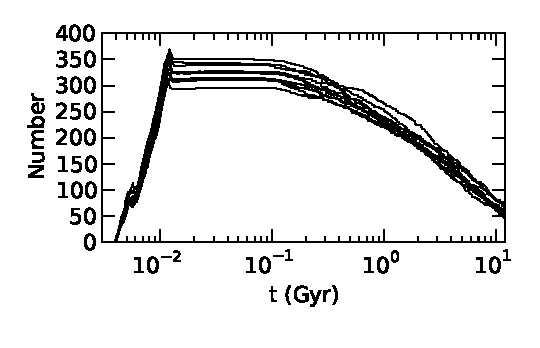
\includegraphics[width=\textwidth]{./plots/r5_repeat10_bh_ret_timevolution.eps}

                \label{fig:repeat10_bhs}
        \end{subfigure}     
        \begin{subfigure}[b]{0.5\textwidth}
                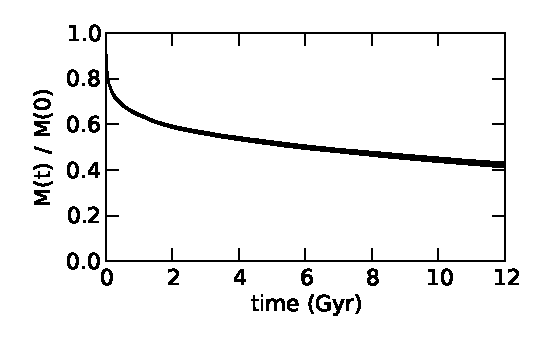
\includegraphics[width=\textwidth]{./plots/r5_repeat10_mass_timeevolution.eps}
                \label{fig:repeat10_mass}
        \end{subfigure}     


	\caption{Statistical fluctuations across 10 realizations of one cluster model - model r5. The total cluster mass, number of BHs as a function of time agree very well across all 10 simulations. \bf{TO DO: plot rc and rh as a function of time for all models - run script over all snapshots}}

\end{figure}


%=======================================================================
%====================     							            ===================
%====================    		     COMPARISON TO	        	   ===================
%====================     		       GALACTIC  GCS 	            ===================
%====================     							            ===================
%=======================================================================


\begin{figure} [!ht]
\epsscale{1.0}

	\plotone{mw_gcs_models_comparison.eps}  
	% To make this figure, from directory with tables (final_properties.dat, my_gc_table_rc_pc.dat)
	%  >>>     extract_model_details.make_MW_histograms()
	\caption{Comparison of observable properties for MW GCs and for our models. The MW data is taken from the \citealt{Harris1996} (2010 edition), excluding the masses, which are from \citealt{Gnedin1997}. The histograms show the distribution of core radii, $r_c$, the ratio of core to half light radius, $r_c\, /\, r_h$, the central luminosity density, $\rho_c$, and total cluster mass, $M$, for the Milky Way GCs (Harris). The ticks show the calculated values for the same quantities for our models. The colors indicate the initial value of $N$. For quantities that depend on \emph{light} (all of the above, except for $M$), we have calculated the quantities with at least two different methods, which are represented by the different sets of ticks at the bottom, center, or top of the plots. For $r_c$ and $r_h$, the ticks on the bottom and top are calculated using the cumulative luminosity function using visual or bolometric luminosities, respectively. The ticks across the middle of the plot of $r_c$ show the values as calculated from the surface brightness profile. For and $\rho$, the bottom set of ticks shows the luminosity density calculated in the visual band within either 0.1 $r_c$ or 0.25 $r_c$, and the two sets of ticks at the top of the panel represent the same quantities as derived from the bolometric luminosities. $M$ is simply the sum of all the masses in the cluster. Our clusters agree well with MW GCs in terms of $\rho_c$ and $M$, but our measured values for $r_c$ and $r_c / r_h$ fall on the high end of the distribution. The three low-$N$ models that dissolved prior to 12 Gyr are excluded from these figures.}

	\label{fig:MW_histograms}
\end{figure}

%\begin{figure}[!h]
%\epsscale{1.0}
%
%	\plotone{mw_rc_vs_M_comparison.eps}
%
%	\caption{$}
%	\label{fig:MW_models_Rc_vs_M}
%\end{figure}

       



%%%%%%%%%%%%%%%%               TABLES           %%%%%%%%%%%%%%%%%





%%%%%%%%%%%%%%%%%%%%%%%%%%%%%%%%%%%%%%%%%%%%
%%%%%%%%%%%%%%%%                                             %%%%%%%%%%%%%%%%
%%%%%%%%%%%%%%%%              IC  TABLE            %%%%%%%%%%%%%%%%
%%%%%%%%%%%%%%%%                                             %%%%%%%%%%%%%%%%
%%%%%%%%%%%%%%%%%%%%%%%%%%%%%%%%%%%%%%%%%%%%


\begin{deluxetable}{ccccccccccc}
%\tablecolumns{7}
\tabletypesize{\scriptsize}
%\tablewidth{0pc}
\tablecaption{Initial model parameters. Columns are as follows: model name, $N$, total mass ($M_{\odot}$), King concentration parameter$W_o$, galactocentric distance $R_G$, metallicity ($Z$), theoretical (code defined) core radius (pc), theoretical half mass radius (pc), initial central mass density ($M_{\odot}/pc^3$), and initial binary fraction.}

\tablehead{
	\colhead{model} & \colhead{$N$} & \colhead{$M$} & \colhead{$W_0$} & \colhead{$R_G$} & \colhead{$Z$}& \colhead{$R_v$} & \colhead{$r_{c,code}$} & \colhead{$r_{h,code}$} & \colhead{$log(\rho_{c})$} & \colhead{$f_{b}$}   \\
\colhead{} & \colhead{$(10^5)$} & \colhead{$(10^5 M_{\odot})$} & \colhead{} & \colhead{(kpc)} & \colhead{} &  \colhead{(pc)} &  \colhead{(pc)}  &  \colhead{(pc)} & \colhead{$(M_{\odot}$/pc$^3)$} & \colhead{}
}

\startdata
%#1:model  #2:N,i(10^5)  #3:M,i(10^5MSun)  #4:Wo  #5:Rg(kpc)  #6:Z  #7:Rv(pc)  #8:rc_theor,i(pc)  #9:rh_theor,i(pc)  #10:log10(rho_c,i)  #11:fb,i
n1w2rg20rv2fb10 & 2.0   & 1.4   & 2     & 20    & 0.0005        & 2     & 1.0   & 1.7   & 4.5   & 0.1 \\
n1w2rg2rv2fb10  & 2.0   & 1.4   & 2     & 2     & 0.005 & 2     & 1.0   & 1.7   & 4.5   & 0.1 \\
n1w2rg8rv2fb10  & 2.0   & 1.4   & 2     & 8     & 0.001 & 2     & 1.0   & 1.7   & 4.5   & 0.1 \\
n1w5rg20rv2fb10 & 2.0   & 1.4   & 5     & 20    & 0.0005        & 2     & 0.7   & 1.6   & 4.7   & 0.1 \\
n1w5rg2rv2fb10  & 2.0   & 1.4   & 5     & 2     & 0.005 & 2     & 0.7   & 1.6   & 4.7   & 0.1 \\
n1w5rg8rv2fb10  & 2.0   & 1.4   & 5     & 8     & 0.001 & 2     & 0.7   & 1.6   & 4.7   & 0.1 \\
n1w7rg20rv2fb10 & 2.0   & 1.4   & 7     & 20    & 0.0005        & 2     & 0.4   & 1.6   & 5.2   & 0.1 \\
n1w7rg2rv2fb10  & 2.0   & 1.4   & 7     & 2     & 0.005 & 2     & 0.4   & 1.6   & 5.2   & 0.1 \\
n1w7rg8rv2fb10  & 2.0   & 1.4   & 7     & 8     & 0.001 & 2     & 0.4   & 1.6   & 5.2   & 0.1 \\
Xn1w11rg8rv2fb10        & 2.0   & 1.4   & 11    & 8     & 0.001 & 2     & 0.1   & 2.0   & 7.4   & 0.1 \\
Xn1w5rg8rv1fb10 & 2.0   & 1.4   & 5     & 8     & 0.001 & 1     & 0.4   & 0.8   & 5.7   & 0.1 \\
Xn1w5rg8rv2fb1  & 2.0   & 1.3   & 5     & 8     & 0.001 & 2     & 0.7   & 1.6   & 4.7   & 0.01 \\
Xn1w5rg8rv2fb50 & 2.0   & 1.7   & 5     & 8     & 0.001 & 2     & 0.7   & 1.6   & 4.8   & 0.5 \\
Xn1w5rg8rv4fb10 & 2.0   & 1.4   & 5     & 8     & 0.001 & 4     & 1.4   & 3.3   & 3.8   & 0.1 \\
\\
n2w2rg20rv2fb10 & 8.0   & 5.4   & 2     & 20    & 0.0005        & 2     & 1.0   & 1.7   & 5.1   & 0.1 \\
n2w2rg2rv2fb10  & 8.0   & 5.4   & 2     & 2     & 0.005 & 2     & 1.0   & 1.7   & 5.1   & 0.1 \\
n2w2rg8rv2fb10  & 8.0   & 5.4   & 2     & 8     & 0.001 & 2     & 1.0   & 1.7   & 5.1   & 0.1 \\
n2w5rg20rv2fb10 & 8.0   & 5.4   & 5     & 20    & 0.0005        & 2     & 0.7   & 1.6   & 5.4   & 0.1 \\
n2w5rg2rv2fb10  & 8.0   & 5.4   & 5     & 2     & 0.005 & 2     & 0.7   & 1.6   & 5.4   & 0.1 \\
n2w5rg8rv2fb10  & 8.0   & 5.4   & 5     & 8     & 0.001 & 2     & 0.7   & 1.6   & 5.4   & 0.1 \\
Xn2w11rg8rv2fb10        & 8.0   & 5.4   & 11    & 8     & 0.001 & 2     & 0.1   & 2.0   & 8.1   & 0.1 \\
Xn2w5rg8rv1fb10 & 8.0   & 5.4   & 5     & 8     & 0.001 & 1     & 0.4   & 0.8   & 6.3   & 0.1 \\
Xn2w5rg8rv2fb1  & 8.0   & 5.1   & 5     & 8     & 0.001 & 2     & 0.7   & 1.6   & 5.4   & 0.01 \\
Xn2w5rg8rv2fb50 & 8.0   & 6.6   & 5     & 8     & 0.001 & 2     & 0.7   & 1.6   & 5.5   & 0.5 \\
Xn2w5rg8rv4fb10 & 8.0   & 5.4   & 5     & 8     & 0.001 & 4     & 1.4   & 3.3   & 4.5   & 0.1 \\
n2w7rg20rv2fb10 & 8.0   & 5.4   & 7     & 20    & 0.0005        & 2     & 0.4   & 1.6   & 5.9   & 0.1 \\
n2w7rg2rv2fb10  & 8.0   & 5.4   & 7     & 2     & 0.005 & 2     & 0.4   & 1.6   & 5.9   & 0.1 \\
n2w7rg8rv2fb10  & 8.0   & 5.4   & 7     & 8     & 0.001 & 2     & 0.4   & 1.6   & 5.9   & 0.1 \\
\\
n3w2rg20rv2fb10 & 16.0  & 10.8  & 2     & 20    & 0.0005        & 2     & 1.0   & 1.7   & 5.4   & 0.1 \\
n3w2rg2rv2fb10  & 16.0  & 10.8  & 2     & 2     & 0.005 & 2     & 1.0   & 1.7   & 5.4   & 0.1 \\
n3w2rg8rv2fb10  & 16.0  & 10.8  & 2     & 8     & 0.001 & 2     & 1.0   & 1.7   & 5.4   & 0.1 \\
n3w5rg20rv2fb10 & 16.0  & 10.8  & 5     & 20    & 0.0005        & 2     & 0.7   & 1.6   & 5.7   & 0.1 \\
n3w5rg2rv2fb10  & 16.0  & 10.8  & 5     & 2     & 0.005 & 2     & 0.7   & 1.6   & 5.7   & 0.1 \\
n3w5rg8rv2fb10  & 16.0  & 10.8  & 5     & 8     & 0.001 & 2     & 0.7   & 1.6   & 5.7   & 0.1 \\
n3w7rg20rv2fb10 & 16.0  & 10.8  & 7     & 20    & 0.0005        & 2     & 0.5   & 1.6   & 6.2   & 0.1 \\
n3w7rg2rv2fb10  & 16.0  & 10.8  & 7     & 2     & 0.005 & 2     & 0.5   & 1.6   & 6.2   & 0.1 \\
n3w7rg8rv2fb10  & 16.0  & 10.8  & 7     & 8     & 0.001 & 2     & 0.5   & 1.6   & 6.2   & 0.1 \\
Xn3w11rg8rv2fb10        & 16.0  & 10.8  & 11    & 8     & 0.001 & 2     & 0.1   & 2.0   & 8.3   & 0.1 \\
Xn3w5rg8rv1fb10 & 16.0  & 10.8  & 5     & 8     & 0.001 & 1     & 0.4   & 0.8   & 6.6   & 0.1 \\
Xn3w5rg8rv2fb1  & 16.0  & 10.3  & 5     & 8     & 0.001 & 2     & 0.7   & 1.6   & 5.6   & 0.01 \\
Xn3w5rg8rv2fb50 & 16.0  & 13.2  & 5     & 8     & 0.001 & 2     & 0.7   & 1.6   & 5.8   & 0.5 \\
Xn3w5rg8rv4fb10 & 16.0  & 10.8  & 5     & 8     & 0.001 & 4     & 1.4   & 3.3   & 4.8   & 0.1 \\




%r1	& n2e5w2r2Rg20z0.0005		& 2.0		& 1.36	& 0.951	& 1.698	& 4.47	& 0.1 \\ 
%r2	& n2e5w2r2Rg8z0.001		& 2.0		& 1.36	& 0.951	& 1.698	& 4.47	& 0.1 \\ 
%r3	& n2e5w2r2Rg2z0.005		& 2.0		& 1.36	& 0.951	& 1.698	& 4.47	& 0.1 \\ 
%r4	& n2e5w5r2Rg20z0.0005		& 2.0		& 1.36	& 0.717	& 1.628	& 4.75	& 0.1 \\ 
%r5	& n2e5w5r2Rg8z0.001		& 2.0		& 1.36	& 0.717	& 1.628	& 4.75	& 0.1 \\ 
%r6	& n2e5w5r2Rg2z0.005		& 2.0		& 1.36	& 0.717	& 1.628	& 4.75	& 0.1 \\ 
%r7	& n2e5w7r2Rg20z0.0005		& 2.0		& 1.36	& 0.449	& 1.624	& 5.25	& 0.1 \\ 
%r8	& n2e5w7r2Rg8z0.001		& 2.0		& 1.36	& 0.449	& 1.624	& 5.25	& 0.1 \\ 
%r9	& n2e5w7r2Rg2z0.005		& 2.0		& 1.36	& 0.449	& 1.624	& 5.25	& 0.1 \\ 
%x22	& n2e5w11r2Rg8z0.001fb0.1	& 2.0		& 1.36	& 0.054	& 2.032	& 7.44	& 0.1 \\ 
%x23	& n2e5w5r4Rg8z0.001fb0.1	& 2.0		& 1.36	& 1.434	& 3.256	& 3.85	& 0.1 \\ 
%x24	& n2e5w5r2Rg8z0.001fb0.01	& 2.0		& 1.29	& 0.717	& 1.631	& 4.71	& 0.01 \\ 
%x25	& n2e5w5r2Rg8z0.001fb0.5	& 2.0		& 1.66	& 0.717	& 1.634	& 4.83	& 0.5 \\ 
%x43	& n2e5w5r1Rg8z0.001fb0.1	& 2.0		& 1.36	& 0.359	& 0.814	& 5.65	& 0.1 \\ 
%r10	& n8e5w2r2Rg20z0.0005		& 8.0		& 5.4		& 0.951	& 1.698	& 5.13	& 0.1 \\ 
%r11	& n8e5w2r2Rg8z0.001		& 8.0		& 5.4		& 0.951	& 1.698	& 5.13	& 0.1 \\ 
%r12	& n8e5w2r2Rg2z0.005		& 8.0		& 5.4		& 0.951	& 1.698	& 5.13	& 0.1 \\ 
%r13	& n8e5w5r2Rg20z0.0005		& 8.0		& 5.4		& 0.716	& 1.627	& 5.43	& 0.1 \\ 
%r14	& n8e5w5r2Rg8z0.001		& 8.0		& 5.4		& 0.716	& 1.627	& 5.43	& 0.1 \\ 
%r15	& n8e5w5r2Rg2z0.005		& 8.0		& 5.4		& 0.716	& 1.627	& 5.43	& 0.1 \\ 
%r16	& n8e5w7r2Rg20z0.0005		& 8.0		& 5.4		& 0.449	& 1.622	& 5.94	& 0.1 \\ 
%r17	& n8e5w7r2Rg8z0.001		& 8.0		& 5.4		& 0.449	& 1.622	& 5.94	& 0.1 \\ 
%r18	& n8e5w7r2Rg2z0.005		& 8.0		& 5.4		& 0.449	& 1.622	& 5.94	& 0.1 \\ 
%x26	& n8e5w11r2Rg8z0.001fb0.1	& 8.0		& 5.4		& 0.055	& 2.024	& 8.08	& 0.1 \\ 
%x27	& n8e5w5r4Rg8z0.001fb0.1	& 8.0		& 5.4		& 1.433	& 3.254	& 4.53	& 0.1 \\ 
%x28	& n8e5w5r2Rg8z0.001fb0.01	& 8.0		& 5.13 	& 0.717	& 1.627	& 5.39	& 0.01 \\ 
%x29	& n8e5w5r2Rg8z0.001fb0.5	& 8.0		& 6.57 	& 0.716	& 1.626	& 5.51	& 0.5 \\ 
%x44	& n8e5w5r1Rg8z0.001fb0.1	& 8.0		& 5.4		& 0.358	& 0.813	& 6.34	& 0.1 \\ 
%r30	& n1.6e6w2r2Rg20z0.0005fb0.1 & 16.0	& 10.82	& 0.954	& 1.7		& 5.38	& 0.1 \\ 
%r31	& n1.6e6w2r2Rg8z0.001fb0.1	& 16.0	& 10.82	& 0.954	& 1.7		& 5.38	& 0.1 \\ 
%r32	& n1.6e6w2r2Rg2z0.005fb0.1	& 16.0	& 10.82	& 0.954	& 1.7		& 5.38	& 0.1 \\ 
%r33	& n1.6e6w5r2Rg20z0.0005fb0.1 & 16.0	& 10.82	& 0.719	& 1.63	& 5.67	& 0.1 \\ 
%r34	& n1.6e6w5r2Rg8z0.001fb0.1	& 16.0	& 10.82	& 0.719	& 1.63	& 5.67	& 0.1 \\ 
%r35	& n1.6e6w5r2Rg2z0.005fb0.1	& 16.0	& 10.82	& 0.719	& 1.63	& 5.67	& 0.1 \\ 
%r36	& n1.6e6w7r2Rg20z0.0005fb0.1 & 16.0	& 10.82	& 0.45	& 1.626	& 6.18	& 0.1 \\ 
%r37	& n1.6e6w7r2Rg8z0.001fb0.1	& 16.0	& 10.82	& 0.45	& 1.626	& 6.18	& 0.1 \\ 
%r38	& n1.6e6w7r2Rg2z0.005fb0.1	& 16.0	& 10.82	& 0.45	& 1.626	& 6.18	& 0.1 \\ 
%x39	& n1.6e6w11r2Rg8z0.001fb0.1 & 16.0	& 10.82	& 0.056	& 2.027	& 8.32	& 0.1 \\ 
%x40	& n1.6e6w5r4Rg8z0.001fb0.1	& 16.0	& 10.82	& 1.439	& 3.259	& 4.77	& 0.1 \\ 
%x41	& n1.6e6w5r2Rg8z0.001fb0.01 & 16.0	& 10.28	& 0.72	& 1.63	& 5.65	& 0.01 \\ 
%x42	& n1.6e6w5r2Rg8z0.001fb0.5	& 16.0	& 13.19	& 0.719	& 1.63	& 5.77	& 0.5 \\ 

\enddata
\label{table:initial_conditions}
\end{deluxetable}


%All models with $N = 2 \times 10^5$ have initial total mass of $M_{\rm tot} = blah \times 10^5\, M_\odot$, and form $\sim xx$ BHs HOW MANY BHS- DO THEY HAVE ROUGHTLY SAME NUMBER FOR EACH N (OR DEPENDS ON METALLICITY). All models with $N = 8 \times 10^5$ have initial total mass of $M_{\rm tot} = blah \times 10^5\, M_\odot$, and form $\sim xx$ BHs. Note that some of the BHs that are formed through stellar evolution are ejected immediately upon formation by a natal kick. Details about the initial population of BHs, including the fraction of BHs retained initially, are given in table ****.








%%%%%%%%%%%%%%%%%%%%%%%%%%%%%%%%%%%%%%%%%%%%
%%%%%%%%%%%%%%%%                                             %%%%%%%%%%%%%%%%
%%%%%%%%%%%%%%%%            T = 12 GYR            %%%%%%%%%%%%%%%%
%%%%%%%%%%%%%%%%                  TABLE              %%%%%%%%%%%%%%%%
%%%%%%%%%%%%%%%%                                             %%%%%%%%%%%%%%%%
%%%%%%%%%%%%%%%%%%%%%%%%%%%%%%%%%%%%%%%%%%%%

\begin{deluxetable}{ccccccccc}
%\tablecolumns{8}
\tabletypesize{\tiny}
%\tablewidth{0pc}
\tablecaption{Cluster properties at 12 Gyr. Columns are as follows: model name, $N$, cluster mass, theoretical (code defined) core radius, theoretical (code defined) half mass radius, log of central mass density, core binary fraction, binary fraction, number of BHs, number of BH-BH binaries, number of binaries consisting of a BH with a non-BH companion, the half-\emph{light} radius, log of central luminosity density}

\tablehead{
\colhead{id} & \colhead{model} & \colhead{$N$} & \colhead{$M$} & \colhead{$r_{c,code}$} & \colhead{$r_{h,code}$} & \colhead{$log(\rho_{c})$} & \colhead{$f_{b}$} & \colhead{$f_{b,core}$}  \\
\colhead{ } & \colhead{} & \colhead{$(10^5)$} & \colhead{$(10^5 M_{\odot})$} & \colhead{(pc)} & \colhead{(pc)} & \colhead{$(M_{\odot}$/pc$^3)$} & \colhead{} & \colhead{}
}

 \startdata
%#1:ID  #2:model  #3:N,f/1e5  #4:M,f/1e5  #5:rc_theor,f  #6:rh_theor,f  #7:log10(rho_c,f)  #8:fb,f  #9:fb,core
r1	& n2e5w2r2Rg20z0.0005		& 1.65	& 0.63	& 3.217	& 8.644	& 2.54	& 0.09	& 0.118 \\ 
r2	& n2e5w2r2Rg8z0.001		& 1.43	& 0.55	& 2.939	& 7.781	& 2.64	& 0.1	& 0.12 \\ 
r3	& n2e5w2r2Rg2z0.005		& 0.04	& 0.03	& 0.034	& 2.632	& 6.2	& 0.16	& 0.167 \\ 
r4	& n2e5w5r2Rg20z0.0005		& 1.68	& 0.64	& 3.112	& 8.944	& 3.08	& 0.09	& 0.113 \\ 
r5	& n2e5w5r2Rg8z0.001		& 1.46	& 0.56	& 3.087	& 8.292	& 2.95	& 0.09	& 0.123 \\ 
r6	& n2e5w5r2Rg2z0.005		& 0.02	& 0.03	& 0.39	& 1.565	& 3.84	& 0.13	& 0.06 \\ 
r7	& n2e5w7r2Rg20z0.0005		& 1.72	& 0.65	& 3.745	& 9.777	& 2.54	& 0.09	& 0.12 \\ 
r8	& n2e5w7r2Rg8z0.001		& 1.44	& 0.56	& 3.521	& 8.938	& 2.74	& 0.09	& 0.123 \\ 
r9	& n2e5w7r2Rg2z0.005		& 0.03	& 0.03	& 0.253	& 1.992	& 4.71	& 0.13	& 0.063 \\ 
x22	& n2e5w11r2Rg8z0.001fb0.1	& 1.28	& 0.5	& 3.786	& 9.437	& 2.69	& 0.1	& 0.114 \\ 
x23	& n2e5w5r4Rg8z0.001fb0.1	& 1.79	& 0.68	& 5.951	& 13.338 & 1.88	& 0.09	& 0.109 \\ 
x24	& n2e5w5r2Rg8z0.001fb0.01	& 1.36	& 0.51	& 3.581	& 8.557	& 2.37	& 0.01	& 0.01 \\ 
x25	& n2e5w5r2Rg8z0.001fb0.5	& 1.55	& 0.71	& 2.592	& 7.616	& 3.62	& 0.47	& 0.54 \\ 
x43	& n2e5w5r1Rg8z0.001fb0.1	& 0.37	& 0.2	& 0.465	& 2.862	& 4.76	& 0.12	& 0.258 \\ 
r10	& n8e5w2r2Rg20z0.0005		& 7.25	& 2.76	& 3.327	& 8.486	& 3.61	& 0.09	& 0.097 \\ 
r11	& n8e5w2r2Rg8z0.001		& 6.86	& 2.62	& 2.174	& 7.939	& 5.23	& 0.09	& 0.102 \\ 
r12	& n8e5w2r2Rg2z0.005		& 5.12	& 2.04	& 2.469	& 6.228	& 3.91	& 0.09	& 0.109 \\ 
r13	& n8e5w5r2Rg20z0.0005		& 7.36	& 2.79	& 3.17	& 8.554	& 3.8	& 0.09	& 0.1 \\ 
r14	& n8e5w5r2Rg8z0.001		& 7.0	& 2.66	& 3.173	& 7.852	& 3.42	& 0.09	& 0.101 \\ 
r15	& n8e5w5r2Rg2z0.005		& 4.99	& 2.0	& 2.744	& 6.603	& 3.69	& 0.09	& 0.107 \\ 
r16	& n8e5w7r2Rg20z0.0005		& 7.41	& 2.81	& 0.023	& 9.251	& 8.98	& 0.09	& 0.048 \\ 
r17	& n8e5w7r2Rg8z0.001		& 7.11	& 2.7	& 3.423	& 8.591	& 3.45	& 0.09	& 0.1 \\ 
r18	& n8e5w7r2Rg2z0.005		& 4.77	& 1.92	& 2.844	& 6.936	& 4.03	& 0.09	& 0.111 \\ 
x26	& n8e5w11r2Rg8z0.001fb0.1	& 6.77	& 2.6	& 2.815	& 9.014	& 4.74	& 0.09	& 0.097 \\ 
x27	& n8e5w5r4Rg8z0.001fb0.1	& 7.6	& 2.91	& 3.901	& 11.748 & 4.44	& 0.09	& 0.097 \\ 
x28	& n8e5w5r2Rg8z0.001fb0.01	& 6.87	& 2.52	& 2.981	& 8.28	& 4.29	& 0.01	& 0.01 \\ 
x29	& n8e5w5r2Rg8z0.001fb0.5	& 7.19	& 3.21	& 2.899	& 7.728	& 3.93	& 0.45	& 0.475 \\ 
x44	& n8e5w5r1Rg8z0.001fb0.1	& 5.56	& 2.17	& 1.687	& 4.906	& 4.28	& 0.09	& 0.119 \\ 
r30	& n1.6e6w2r2Rg20z0.0005fb0.1	& 14.82	& 5.68	& 2.962	& 8.013	& 4.32	& 0.09	& 0.092 \\ 
r31	& n1.6e6w2r2Rg8z0.001fb0.1	& 14.39	& 5.5	& 1.614	& 7.456	& 6.16	& 0.09	& 0.093 \\ 
r32	& n1.6e6w2r2Rg2z0.005fb0.1	& 12.38	& 4.84	& 1.421	& 6.426	& 6.47	& 0.09	& 0.1 \\ 
r33	& n1.6e6w5r2Rg20z0.0005fb0.1	& 14.82	& 5.76	& 0.013	& 8.511	& 10.1	& 0.09	& 0.25 \\ 
r34	& n1.6e6w5r2Rg8z0.001fb0.1	& 14.54	& 5.56	& 2.412	& 7.823	& 5.42	& 0.09	& 0.095 \\ 
r35	& n1.6e6w5r2Rg2z0.005fb0.1	& 12.77	& 4.97	& 2.119	& 6.581	& 5.34	& 0.09	& 0.101 \\ 
r36	& n1.6e6w7r2Rg20z0.0005fb0.1	& 15.11	& 5.76	& 2.873	& 8.772	& 4.69	& 0.09	& 0.09 \\ 
r37	& n1.6e6w7r2Rg8z0.001fb0.1	& 14.61	& 5.58	& 2.773	& 8.419	& 4.98	& 0.09	& 0.093 \\ 
r38	& n1.6e6w7r2Rg2z0.005fb0.1	& 12.79	& 4.96	& 2.859	& 7.104	& 4.08	& 0.09	& 0.1 \\ 
x39	& n1.6e6w11r2Rg8z0.001fb0.1	& 14.23	& 5.47	& 3.26	& 8.484	& 3.93	& 0.09	& 0.092 \\ 
x40	& n1.6e6w5r4Rg8z0.001fb0.1	& 15.46	& 5.94	& 4.821	& 11.138 & 3.67	& 0.09	& 0.094 \\ 
x41	& n1.6e6w5r2Rg8z0.001fb0.01	& 14.38	& 5.28	& 2.86	& 7.774	& 4.48	& 0.01	& 0.009 \\ 
x42	& n1.6e6w5r2Rg8z0.001fb0.5	& 14.8	& 6.63	& 3.033	& 7.552	& 4.04	& 0.45	& 0.45 \\ 

\enddata
\label{table:final_properties}
\end{deluxetable}






%%%%%%%%%%%%%%%%%%%%%%%%%%%%%%%%%%%%%%%%%%%%
%%%%%%%%%%%%%%%%                                             %%%%%%%%%%%%%%%%
%%%%%%%%%%%%%%%%       OBSERVABLES         %%%%%%%%%%%%%%%%
%%%%%%%%%%%%%%%%                TABLE                %%%%%%%%%%%%%%%%
%%%%%%%%%%%%%%%%                                             %%%%%%%%%%%%%%%%
%%%%%%%%%%%%%%%%%%%%%%%%%%%%%%%%%%%%%%%%%%%%

%%%%%%%%%%   OBSERVATIONAL QUANTITIES TABLE    %%%%%%%%%%%
\begin{deluxetable}{ccccccccccc}
\tabletypesize{\tiny}
\tablecaption{Observational quantities for all models, including the core radius $r_c$ (pc), half-light radius $r_h$ (pc) and $r_c/r_h$, and central luminosity density. The first two columns designate the model. The next four columns show the quantities as measured
with the cumulative luminosity function using bolometric luminosities. This is followed by the same four values measured using
visual luminosities. The last column is the core radius as calculated from the surface brightness profile. The methods used for calculating these quantities is described in section \textbf{FILL IN SECTION NAME}.}
\tablehead{
	\colhead{id} & \colhead{model} & \multicolumn{4}{c}{bolometric}  & \multicolumn{4}{c}{visual}  & \colhead{SBP} \\
	\colhead{} & \colhead{} &
	\colhead{$r_c$} & \colhead{$r_h$} & \colhead{$r_c/r_h$} & \colhead{$\rho_l$} & 
	\colhead{$r_c$} & \colhead{$r_h$} & \colhead{$r_c/r_h$} & \colhead{$\rho_l$} & 
	\colhead{$r_c$}
}
	
\startdata
%#  1:ID   2:Model   Bol (3:Rc   4:Rh   5:Rc/Rh   6:rho)   V (7:Rc   8:Rh   9:Rc/Rh   10:rho)   11:Rc(SBP)
r1 & n2e5w2r2Rg20z0.0005 & 3.34 & 6.85 & 0.49 & 3.54 & 2.09 & 5.16 & 0.41 & 3.47 & 1.85 \\ 
r2 & n2e5w2r2Rg8z0.001 & 3.22 & 6.19 & 0.52 & 3.62 & 3.4 & 4.41 & 0.77 & 3.38 & 3.01 \\ 
r3 & n2e5w2r2Rg2z0.005 & 2.43 & 3.18 & 0.76 & 3.59 & 1.36 & 3.13 & 0.43 & 3.77 & 2.9 \\ 
r4 & n2e5w5r2Rg20z0.0005 & 3.28 & 7.15 & 0.46 & 3.59 & 3.1 & 5.88 & 0.53 & 3.44 & 3.9 \\ 
r5 & n2e5w5r2Rg8z0.001 & 3.3 & 6.54 & 0.5 & 3.6 & 4.75 & 4.24 & 1.12 & 3.59 & 3.0 \\ 
r6 & n2e5w5r2Rg2z0.005 & 2.98 & 3.88 & 0.77 & 3.69 & 2.65 & 3.37 & 0.78 & 3.9 & 2.86 \\ 
r7 & n2e5w7r2Rg20z0.0005 & 4.29 & 7.82 & 0.55 & 3.3 & 2.75 & 6.14 & 0.45 & 3.18 & 2.84 \\ 
r8 & n2e5w7r2Rg8z0.001 & 3.72 & 7.08 & 0.53 & 3.8 & 2.8 & 6.01 & 0.47 & 3.87 & 4.55 \\ 
r9 & n2e5w7r2Rg2z0.005 & 2.92 & 3.88 & 0.75 & 3.9 & 2.36 & 3.38 & 0.7 & 4.09 & 2.13 \\ 
x22 & n2e5w11r2Rg8z0.001fb0.1 & 4.73 & 7.47 & 0.63 & 3.17 & 6.65 & 6.69 & 0.99 & 2.64 & 3.39 \\ 
x23 & n2e5w5r4Rg8z0.001fb0.1 & 6.26 & 10.41 & 0.6 & 2.94 & 5.36 & 9.19 & 0.58 & 3.12 & 7.35 \\ 
x24 & n2e5w5r2Rg8z0.001fb0.01 & 3.92 & 6.86 & 0.57 & 3.46 & 4.69 & 4.48 & 1.05 & 3.42 & 3.38 \\ 
x25 & n2e5w5r2Rg8z0.001fb0.5 & 2.58 & 5.43 & 0.47 & 3.79 & 1.32 & 3.77 & 0.35 & 4.07 & 2.04 \\ 
x43 & n2e5w5r1Rg8z0.001fb0.1 & 0.53 & 2.26 & 0.23 & 5.4 & 0.5 & 1.5 & 0.34 & 5.21 & 0.37 \\ 
r10 & n8e5w2r2Rg20z0.0005 & 3.95 & 6.86 & 0.58 & 4.07 & 3.13 & 6.03 & 0.52 & 3.75 & 3.65 \\ 
r11 & n8e5w2r2Rg8z0.001 & 3.82 & 6.36 & 0.6 & 4.14 & 3.33 & 5.73 & 0.58 & 4.0 & 2.99 \\ 
r12 & n8e5w2r2Rg2z0.005 & 3.06 & 4.96 & 0.62 & 4.38 & 2.51 & 3.99 & 0.63 & 4.45 & 2.18 \\ 
r13 & n8e5w5r2Rg20z0.0005 & 4.04 & 6.91 & 0.59 & 4.08 & 3.56 & 6.04 & 0.59 & 3.91 & 4.3 \\ 
r14 & n8e5w5r2Rg8z0.001 & 3.73 & 6.25 & 0.6 & 4.2 & 2.18 & 5.35 & 0.41 & 4.29 & 2.97 \\ 
r15 & n8e5w5r2Rg2z0.005 & 3.44 & 5.23 & 0.66 & 4.21 & 2.2 & 4.21 & 0.52 & 4.02 & 3.21 \\ 
r16 & n8e5w7r2Rg20z0.0005 & 4.48 & 7.45 & 0.6 & 3.98 & 4.91 & 6.39 & 0.77 & 3.67 & 3.74 \\ 
r17 & n8e5w7r2Rg8z0.001 & 4.04 & 6.9 & 0.59 & 4.05 & 3.27 & 6.59 & 0.5 & 3.86 & 3.0 \\ 
r18 & n8e5w7r2Rg2z0.005 & 3.65 & 5.47 & 0.67 & 4.23 & 3.41 & 4.44 & 0.77 & 4.05 & 2.13 \\ 
x26 & n8e5w11r2Rg8z0.001fb0.1 & 4.34 & 7.17 & 0.6 & 3.98 & 4.19 & 6.24 & 0.67 & 3.78 & 3.47 \\ 
x27 & n8e5w5r4Rg8z0.001fb0.1 & 6.57 & 9.45 & 0.7 & 3.53 & 4.91 & 8.03 & 0.61 & 3.34 & 7.5 \\ 
x28 & n8e5w5r2Rg8z0.001fb0.01 & 4.23 & 6.65 & 0.64 & 4.05 & 3.43 & 5.66 & 0.61 & 3.97 & 4.66 \\ 
x29 & n8e5w5r2Rg8z0.001fb0.5 & 3.12 & 5.88 & 0.53 & 4.25 & 2.76 & 4.99 & 0.55 & 4.29 & 2.65 \\ 
x44 & n8e5w5r1Rg8z0.001fb0.1 & 1.85 & 3.94 & 0.47 & 4.93 & 1.41 & 3.05 & 0.46 & 4.91 & 1.27 \\ 
r30 & n1.6e6w2r2Rg20z0.0005fb0.1 & 3.96 & 6.47 & 0.61 & 4.41 & 3.3 & 5.76 & 0.57 & 4.33 & 4.1 \\ 
r31 & n1.6e6w2r2Rg8z0.001fb0.1 & 3.72 & 6.02 & 0.62 & 4.49 & 3.12 & 5.55 & 0.56 & 4.33 & 3.39 \\ 
r32 & n1.6e6w2r2Rg2z0.005fb0.1 & 3.3 & 5.12 & 0.64 & 4.65 & 3.27 & 4.34 & 0.75 & 4.58 & 2.57 \\ 
r33 & n1.6e6w5r2Rg20z0.0005fb0.1 & 4.25 & 6.92 & 0.61 & 4.36 & 3.87 & 6.46 & 0.6 & 4.29 & 3.43 \\ 
r34 & n1.6e6w5r2Rg8z0.001fb0.1 & 4.03 & 6.28 & 0.64 & 4.43 & 3.71 & 5.64 & 0.66 & 4.24 & 3.99 \\ 
r35 & n1.6e6w5r2Rg2z0.005fb0.1 & 3.34 & 5.25 & 0.64 & 4.64 & 2.57 & 4.48 & 0.57 & 4.64 & 2.96 \\ 
r36 & n1.6e6w7r2Rg20z0.0005fb0.1 & 4.32 & 7.07 & 0.61 & 4.31 & 3.68 & 6.52 & 0.56 & 4.09 & 4.14 \\ 
r37 & n1.6e6w7r2Rg8z0.001fb0.1 & 4.31 & 6.74 & 0.64 & 4.34 & 4.11 & 6.14 & 0.67 & 4.11 & 4.65 \\ 
r38 & n1.6e6w7r2Rg2z0.005fb0.1 & 3.59 & 5.63 & 0.64 & 4.54 & 3.07 & 4.85 & 0.63 & 4.42 & 2.44 \\ 
x39 & n1.6e6w11r2Rg8z0.001fb0.1 & 4.2 & 6.76 & 0.62 & 4.36 & 3.8 & 6.23 & 0.61 & 4.28 & 3.97 \\ 
x40 & n1.6e6w5r4Rg8z0.001fb0.1 & 6.77 & 8.97 & 0.75 & 3.84 & 6.75 & 8.5 & 0.79 & 3.6 & 7.24 \\ 
x41 & n1.6e6w5r2Rg8z0.001fb0.01 & 4.05 & 6.28 & 0.64 & 4.44 & 4.0 & 5.59 & 0.71 & 4.24 & 3.95 \\ 
x42 & n1.6e6w5r2Rg8z0.001fb0.5 & 3.45 & 5.82 & 0.59 & 4.47 & 3.33 & 5.12 & 0.65 & 4.32 & 3.0 \\ 
\enddata
\label{table:Observables}
\vspace{-0.6cm}
\tablecomments{All radii are in units of pc. The central luminosity density, $\rho_l$, is given in units of $L_{\odot, \rm x}/\rm pc^3$, where x is either the Sun's bolometric or v-band luminosity. Columns 2-5 are calculated using the bolometric luminosities of stars as determined by BSE, while columns 6-9 use v-band luminosities as described in the text. The last column is calculated from the SBP using v-band magnitudes. \bf{Should details like excluding stars brighter than mag 3, and number of bins, etc. for SBP be described here, or in the text?}}
\end{deluxetable}


%%%%%%%%%%%%%%%%%%%%%%%%%%%%%%%%%%%%%%%%%%%%
%%%%%%%%%%%%%%%%                                             %%%%%%%%%%%%%%%%
%%%%%%%%%%%%%%%%         EXTRA STUFF         %%%%%%%%%%%%%%%%
%%%%%%%%%%%%%%%%       OBSERVABLES         %%%%%%%%%%%%%%%%
%%%%%%%%%%%%%%%%                TABLE                %%%%%%%%%%%%%%%%
%%%%%%%%%%%%%%%%                                             %%%%%%%%%%%%%%%%
%%%%%%%%%%%%%%%%%%%%%%%%%%%%%%%%%%%%%%%%%%%%

%\begin{deluxetable}{ccccccccccccccccccccc}
%\rotate
% %\begin{adjustwidth}{-2cm}{}
%\tabletypesize{\tiny}
%\tablecaption{Observational quantities for all models, including the core radius $r_c$ (pc), half-light radius $r_h$ (pc) and $r_c/r_h$, and central luminosity density. Method used for calculating these quantities is described in section BLAH.}
%\tablehead{
%	\colhead{id} & \colhead{model} & \colhead{$r_c$(SBP)} & 
%	\colhead{$r_c$(V)} & \colhead{$r_c$(bol)} & 
%	\colhead{$r_h$(V)} & \colhead{$r_h$(bol)} & 
%	\colhead{$r_c/r_h$(V)} & \colhead{$r_c/r_h$(bol)} &
%	\colhead{log($\rho_v$(0.1 $r_c$} & \colhead{log($\rho_bol$(0.1 $r_c$} &
%	\colhead{$N(L_v, 0.1 r_c$} & \colhead{$N(L_bol, 0.1 r_c$} &
%	\colhead{log($\rho_v$(0.1 $r_c$} & \colhead{log($\rho_bol$(0.1 $r_c$} &
%	\colhead{$N(L_v, 0.25 r_c$} & \colhead{$N(L_bol, 0.25 r_c$} &
%	\colhead{log($\rho_v$(0.25 $r_c$} & \colhead{log($\rho_bol$(0.25 $r_c$} &
%	\colhead{$N(L_v, 0.5 r_c$} & \colhead{$N(L_bol, 0.5 r_c$} 
%}
%
%\startdata
%%#0:id  1:model #2:rc(SBP) #3:rc(V) #4:rc(bol) #5:rh(V) #6:rh(bol) #7:rc/rh(V) #8:rc/rh(bol) #9:log10(rho_L_V(0.1*rc)) #10:log10(rho_L_bol(0.1*rc)) #11:N_(LV,0.1*pc) #12:N_(Lbol,0.1*pc) #13:log10(rho_L_V(0.25*rc)) #14:log10(rho_L_bol(0.25*rc)) #15:N_(LV,0.25*pc) #16:N_(Lbol,0.25*pc) #17:log10(rho_L_V(0.5*rc)) #18:log10(rho_L_bol(0.5*rc)) #19:N_(LV,0.5*pc) #20::N_(Lbol,0.5*pc)
%
%r1 & n2e5w2r2Rg20z0.0005 & 1.85 & 2.09 & 3.34 & 5.16 & 6.85 & 0.41 & 0.49 & 3.47 & 3.54 & 247 & 576 & 2.93 & 2.8 & 4779 & 10948 & 2.58 & 2.4 & 16154 & 34336 \\ 
%r2 & n2e5w2r2Rg8z0.001 & 3.01 & 3.4 & 3.22 & 4.41 & 6.19 & 0.77 & 0.52 & 3.38 & 3.62 & 616 & 552 & 2.76 & 2.83 & 11342 & 10312 & 2.39 & 2.43 & 34705 & 32013 \\ 
%r3 & n2e5w2r2Rg2z0.005 & 2.9 & 1.36 & 2.43 & 3.13 & 3.18 & 0.43 & 0.76 & 3.77 & 3.59 & 66 & 167 & 3.76 & 2.86 & 905 & 2535 & 3.18 & 2.49 & 3095 & 8323 \\ 
%r4 & n2e5w5r2Rg20z0.0005 & 3.9 & 3.1 & 3.28 & 5.88 & 7.15 & 0.53 & 0.46 & 3.44 & 3.59 & 489 & 535 & 2.72 & 2.86 & 9186 & 10138 & 2.22 & 2.4 & 29560 & 32203 \\ 
%r5 & n2e5w5r2Rg8z0.001 & 3.0 & 4.75 & 3.3 & 4.24 & 6.54 & 1.12 & 0.5 & 3.59 & 3.6 & 1021 & 524 & 2.56 & 2.82 & 18041 & 9593 & 2.11 & 2.38 & 51314 & 30565 \\ 
%r6 & n2e5w5r2Rg2z0.005 & 2.86 & 2.65 & 2.98 & 3.37 & 3.88 & 0.78 & 0.77 & 3.9 & 3.69 & 285 & 341 & 3.09 & 2.88 & 4602 & 5734 & 2.87 & 2.5 & 15605 & 18947 \\ 
%r7 & n2e5w7r2Rg20z0.0005 & 2.84 & 2.75 & 4.29 & 6.14 & 7.82 & 0.45 & 0.55 & 3.18 & 3.3 & 319 & 678 & 2.63 & 2.56 & 6186 & 13644 & 2.32 & 2.14 & 20989 & 42251 \\ 
%r8 & n2e5w7r2Rg8z0.001 & 4.55 & 2.8 & 3.72 & 6.01 & 7.08 & 0.47 & 0.53 & 3.87 & 3.8 & 317 & 519 & 2.71 & 2.66 & 6097 & 10113 & 2.39 & 2.24 & 20399 & 32190 \\ 
%r9 & n2e5w7r2Rg2z0.005 & 2.13 & 2.36 & 2.92 & 3.38 & 3.88 & 0.7 & 0.75 & 4.09 & 3.9 & 189 & 277 & 3.33 & 2.89 & 3322 & 4872 & 3.04 & 2.5 & 11359 & 16233 \\ 
%x22 & n2e5w11r2Rg8z0.001fb0.1 & 3.39 & 6.65 & 4.73 & 6.69 & 7.47 & 0.99 & 0.63 & 2.64 & 3.17 & 1178 & 623 & 1.95 & 2.38 & 21507 & 12009 & 1.56 & 1.97 & 58751 & 37284 \\ 
%x23 & n2e5w5r4Rg8z0.001fb0.1 & 7.35 & 5.36 & 6.26 & 9.19 & 10.41 & 0.58 & 0.6 & 3.12 & 2.94 & 514 & 676 & 1.95 & 2.08 & 10698 & 14154 & 1.69 & 1.74 & 36269 & 46390 \\ 
%x24 & n2e5w5r2Rg8z0.001fb0.01 & 3.38 & 4.69 & 3.92 & 4.48 & 6.86 & 1.05 & 0.57 & 3.42 & 3.46 & 696 & 500 & 2.53 & 2.6 & 13667 & 9978 & 2.11 & 2.21 & 41038 & 31611 \\ 
%x25 & n2e5w5r2Rg8z0.001fb0.5 & 2.04 & 1.32 & 2.58 & 3.77 & 5.43 & 0.35 & 0.47 & 4.07 & 3.79 & 170 & 555 & 3.21 & 3.04 & 3316 & 11199 & 3.24 & 2.62 & 11648 & 35236 \\ 
%x43 & n2e5w5r1Rg8z0.001fb0.1 & 0.37 & 0.5 & 0.53 & 1.5 & 2.26 & 0.34 & 0.23 & 5.21 & 5.4 & 95 & 106 & 4.64 & 4.49 & 1364 & 1462 & 4.07 & 3.98 & 3863 & 4105 \\ 
%r10 & n8e5w2r2Rg20z0.0005 & 3.65 & 3.13 & 3.95 & 6.03 & 6.86 & 0.52 & 0.58 & 3.75 & 4.07 & 2067 & 3192 & 3.34 & 3.3 & 40584 & 61310 & 2.85 & 2.9 & 134129 & 191610 \\ 
%r11 & n8e5w2r2Rg8z0.001 & 2.99 & 3.33 & 3.82 & 5.73 & 6.36 & 0.58 & 0.6 & 4.0 & 4.14 & 2563 & 3235 & 3.3 & 3.35 & 47501 & 60546 & 2.88 & 2.94 & 153469 & 188567 \\ 
%r12 & n8e5w2r2Rg2z0.005 & 2.18 & 2.51 & 3.06 & 3.99 & 4.96 & 0.63 & 0.62 & 4.45 & 4.38 & 1698 & 2459 & 3.61 & 3.56 & 32119 & 45394 & 3.12 & 3.14 & 104376 & 141447 \\ 
%r13 & n8e5w5r2Rg20z0.0005 & 4.3 & 3.56 & 4.04 & 6.04 & 6.91 & 0.59 & 0.59 & 3.91 & 4.08 & 2704 & 3389 & 3.2 & 3.29 & 51261 & 64136 & 2.76 & 2.88 & 164569 & 199184 \\ 
%r14 & n8e5w5r2Rg8z0.001 & 2.97 & 2.18 & 3.73 & 5.35 & 6.25 & 0.41 & 0.6 & 4.29 & 4.2 & 1134 & 3167 & 3.78 & 3.4 & 23148 & 61293 & 3.32 & 2.97 & 80390 & 190563 \\ 
%r15 & n8e5w5r2Rg2z0.005 & 3.21 & 2.2 & 3.44 & 4.21 & 5.23 & 0.52 & 0.66 & 4.02 & 4.21 & 1043 & 2511 & 3.63 & 3.43 & 21155 & 47358 & 3.22 & 3.01 & 72597 & 148419 \\ 
%r16 & n8e5w7r2Rg20z0.0005 & 3.74 & 4.91 & 4.48 & 6.39 & 7.45 & 0.77 & 0.6 & 3.67 & 3.98 & 4235 & 3567 & 2.89 & 3.17 & 78368 & 66854 & 2.5 & 2.76 & 236737 & 207592 \\ 
%r17 & n8e5w7r2Rg8z0.001 & 3.0 & 3.27 & 4.04 & 6.59 & 6.9 & 0.5 & 0.59 & 3.86 & 4.05 & 2165 & 3202 & 3.26 & 3.29 & 42228 & 61481 & 2.84 & 2.87 & 138784 & 191588 \\ 
%r18 & n8e5w7r2Rg2z0.005 & 2.13 & 3.41 & 3.65 & 4.44 & 5.47 & 0.77 & 0.67 & 4.05 & 4.23 & 2117 & 2409 & 3.19 & 3.33 & 40392 & 45576 & 2.8 & 2.92 & 129579 & 143993 \\ 
%x26 & n8e5w11r2Rg8z0.001fb0.1 & 3.47 & 4.19 & 4.34 & 6.24 & 7.17 & 0.67 & 0.6 & 3.78 & 3.98 & 3081 & 3283 & 3.08 & 3.19 & 57464 & 61082 & 2.65 & 2.77 & 180165 & 189792 \\ 
%x27 & n8e5w5r4Rg8z0.001fb0.1 & 7.5 & 4.91 & 6.57 & 8.03 & 9.45 & 0.61 & 0.7 & 3.34 & 3.53 & 2508 & 4231 & 2.84 & 2.77 & 47852 & 80890 & 2.42 & 2.35 & 161186 & 253493 \\ 
%x28 & n8e5w5r2Rg8z0.001fb0.01 & 4.66 & 3.43 & 4.23 & 5.66 & 6.65 & 0.61 & 0.64 & 3.97 & 4.05 & 2209 & 3220 & 3.31 & 3.27 & 42129 & 61243 & 2.86 & 2.86 & 137933 & 190014 \\ 
%x29 & n8e5w5r2Rg8z0.001fb0.5 & 2.65 & 2.76 & 3.12 & 4.99 & 5.88 & 0.55 & 0.53 & 4.29 & 4.25 & 2652 & 3317 & 3.51 & 3.48 & 51166 & 63722 & 3.08 & 3.06 & 168420 & 203980 \\ 
%x44 & n8e5w5r1Rg8z0.001fb0.1 & 1.27 & 1.41 & 1.85 & 3.05 & 3.94 & 0.46 & 0.47 & 4.91 & 4.93 & 1187 & 1986 & 4.31 & 4.11 & 22597 & 36775 & 3.83 & 3.69 & 73768 & 112791 \\ 
%r30 & n1.6e6w2r2Rg20z0.0005fb0.1 & 4.1 & 3.3 & 3.96 & 5.76 & 6.47 & 0.57 & 0.61 & 4.33 & 4.41 & 5100 & 7050 & 3.56 & 3.64 & 98813 & 136401 & 3.14 & 3.23 & 322759 & 424991 \\ 
%r31 & n1.6e6w2r2Rg8z0.001fb0.1 & 3.39 & 3.12 & 3.72 & 5.55 & 6.02 & 0.56 & 0.62 & 4.33 & 4.49 & 5120 & 6923 & 3.63 & 3.72 & 97417 & 133095 & 3.26 & 3.31 & 318349 & 415511 \\ 
%r32 & n1.6e6w2r2Rg2z0.005fb0.1 & 2.57 & 3.27 & 3.3 & 4.34 & 5.12 & 0.75 & 0.64 & 4.58 & 4.65 & 6152 & 6244 & 3.62 & 3.85 & 116610 & 118301 & 3.25 & 3.44 & 364579 & 369054 \\ 
%r33 & n1.6e6w5r2Rg20z0.0005fb0.1 & 3.43 & 3.87 & 4.25 & 6.46 & 6.92 & 0.6 & 0.61 & 4.29 & 4.36 & 6417 & 7523 & 3.44 & 3.54 & 118334 & 139429 & 3.06 & 3.13 & 375366 & 431358 \\ 
%r34 & n1.6e6w5r2Rg8z0.001fb0.1 & 3.99 & 3.71 & 4.03 & 5.64 & 6.28 & 0.66 & 0.64 & 4.24 & 4.43 & 6410 & 7444 & 3.49 & 3.64 & 122232 & 141619 & 3.11 & 3.23 & 387395 & 438581 \\ 
%r35 & n1.6e6w5r2Rg2z0.005fb0.1 & 2.96 & 2.57 & 3.34 & 4.48 & 5.25 & 0.57 & 0.64 & 4.64 & 4.64 & 3961 & 6322 & 3.82 & 3.84 & 75966 & 120543 & 3.42 & 3.43 & 250383 & 374857 \\ 
%r36 & n1.6e6w7r2Rg20z0.0005fb0.1 & 4.14 & 3.68 & 4.32 & 6.52 & 7.07 & 0.56 & 0.61 & 4.09 & 4.31 & 5544 & 7323 & 3.39 & 3.53 & 105082 & 139435 & 3.02 & 3.12 & 340317 & 433563 \\ 
%r37 & n1.6e6w7r2Rg8z0.001fb0.1 & 4.65 & 4.11 & 4.31 & 6.14 & 6.74 & 0.67 & 0.64 & 4.11 & 4.34 & 6803 & 7439 & 3.36 & 3.55 & 131160 & 142738 & 2.98 & 3.14 & 412156 & 442058 \\ 
%r38 & n1.6e6w7r2Rg2z0.005fb0.1 & 2.44 & 3.07 & 3.59 & 4.85 & 5.63 & 0.63 & 0.64 & 4.42 & 4.54 & 4755 & 6301 & 3.66 & 3.75 & 92287 & 121756 & 3.22 & 3.34 & 297000 & 376901 \\ 
%x39 & n1.6e6w11r2Rg8z0.001fb0.1 & 3.97 & 3.8 & 4.2 & 6.23 & 6.76 & 0.61 & 0.62 & 4.28 & 4.36 & 5912 & 7052 & 3.41 & 3.56 & 113268 & 134793 & 3.03 & 3.15 & 359629 & 416787 \\ 
%x40 & n1.6e6w5r4Rg8z0.001fb0.1 & 7.24 & 6.75 & 6.77 & 8.5 & 8.97 & 0.79 & 0.75 & 3.6 & 3.84 & 9076 & 9141 & 2.84 & 3.07 & 183529 & 184720 & 2.44 & 2.66 & 571962 & 574824 \\ 
%x41 & n1.6e6w5r2Rg8z0.001fb0.01 & 3.95 & 4.0 & 4.05 & 5.59 & 6.28 & 0.71 & 0.64 & 4.24 & 4.44 & 6732 & 6874 & 3.45 & 3.65 & 129187 & 131895 & 3.05 & 3.24 & 402272 & 409283 \\ 
%x42 & n1.6e6w5r2Rg8z0.001fb0.5 & 3.0 & 3.33 & 3.45 & 5.12 & 5.82 & 0.65 & 0.59 & 4.32 & 4.47 & 7360 & 7876 & 3.65 & 3.7 & 147391 & 157513 & 3.23 & 3.28 & 470214 & 497520 \\ 
%\enddata
%\label{table:core_radii}
%\vspace{-0.6cm}
%\tablecomments{All radii are in units of pc. The central luminosity density, $\rho_l$, is given in units of $L_{\odot, \rm x}/\rm pc^3$, where x is either the Sun's bolometric or v-band luminosity. Columns 2-5 are calculated using the bolometric luminosities of stars as determined by BSE, while columns 6-9 use v-band luminosities as described in the text. The last column is calculated from the SBP using v-band magnitudes. \bf{Should details like excluding stars brighter than mag 3, and number of bins, etc. for SBP be described here, or in the text?}}
%% \end{adjustwidth}
%\end{deluxetable}





%%%%%%%%%%%%%%%%%%%%%%%%%%%%%%%%%%%%%%%%%%%%
%%%%%%%%%%%%%%%%                                             %%%%%%%%%%%%%%%%
%%%%%%%%%%%%%%%%            RETAINED             %%%%%%%%%%%%%%%%
%%%%%%%%%%%%%%%%            BHs  TABLE           %%%%%%%%%%%%%%%%
%%%%%%%%%%%%%%%%                                             %%%%%%%%%%%%%%%%
%%%%%%%%%%%%%%%%%%%%%%%%%%%%%%%%%%%%%%%%%%%%

\begin{deluxetable}{cc|cccccccc}
\tabletypesize{\scriptsize}
\tablecaption{Numbers of BHs and various types of BH binaries at the end of each simulation.  The first column gives the name of the model. The next two columns show the name of the model. The next two columns give the total number of BHs that formed and the total number retained at the end of the simulation. The rest of the columns give the numbers of different types of BH objects retained in the cluster at 12 Gyr.}
%% BH table headings
\tablehead{
\colhead{id} & \colhead{model} & \colhead{BH} & \colhead{BH} & \colhead{single} & \colhead{BH-BH} & \colhead{BH-other} & \colhead{BH-NS} & \colhead{BH-WD} & \colhead{BH-star} \\
%\colhead{id} & \colhead{model} & \colhead{$N_{bh}$} & \colhead{$N_{bh}$} & \colhead{$N_{bh,s}$} & \colhead{$N_{bh-bh}$} & \colhead{$N_{bh-other}$} & \colhead{$N_{bh-ns}$} & \colhead{$N_{bh-wd}$} & \colhead{$N_{bh\-star}$} 
\colhead{} & \colhead{} & \colhead{initial} & \colhead{final} & \colhead{} & \colhead{} & \colhead{} & \colhead{} & \colhead{} & \colhead{}
}


\startdata

r1	& n2e5w2r2Rg20z0.0005	 & 474		& 76		& 74		& 1	& 0	& 0	& 0	& 0	\\%& 0.013 \\ 
r2	& n2e5w2r2Rg8z0.001	& 459		& 58		& 57		& 0	& 1	& 0	& 0	& 1	\\%& 0.017 \\ 
r3	& n2e5w2r2Rg2z0.005	& 430		& 81		& 76		& 2	& 1	& 0	& 0	& 1	\\%& 0.038 \\ 
r4	& n2e5w5r2Rg20z0.0005	& 471		& 73		& 71		& 1	& 0	& 0	& 0	& 0	\\%& 0.014 \\ 
r5	& n2e5w5r2Rg8z0.001	& 457		& 65		& 61		& 2	& 0	& 0	& 0	& 0	\\%& 0.032 \\ 
r6	& n2e5w5r2Rg2z0.005	& 427		& 111	& 110	& 0	& 1	& 0	& 0	& 1	\\%& 0.009 \\ 
r7	& n2e5w7r2Rg20z0.0005	& 477		& 82		& 77		& 2	& 1	& 0	& 0	& 1	\\%& 0.037 \\ 
r8	& n2e5w7r2Rg8z0.001	& 459		& 66		& 62		& 2	& 0	& 0	& 0	& 0	\\%& 0.031 \\ 
r9	& n2e5w7r2Rg2z0.005	& 433		& 116	& 111	& 2	& 1	& 0	& 0	& 1	\\%& 0.026 \\ 
x22	& n2e5w11r2Rg8z0.001fb0.1	& 464	& 76		& 72		& 1	& 2	& 0	& 1	& 1	\\%& 0.04 \\ 
x23	& n2e5w5r4Rg8z0.001fb0.1	& 454	& 135	& 128	& 3	& 1	& 0	& 0	& 1	\\%& 0.03 \\ 
x24	& n2e5w5r2Rg8z0.001fb0.01	& 456	& 74		& 70		& 2	& 0	& 0	& 0	& 0	\\%& 0.028 \\ 
x25	& n2e5w5r2Rg8z0.001fb0.5	& 472	& 47		& 44		& 1	& 1	& 0	& 0	& 1	\\%& 0.043 \\ 
x43	& n2e5w5r1Rg8z0.001fb0.1	& 463	& 9		& 9		& 0	& 0	& 0	& 0	& 0	\\%& 0.0 \\ 
r10	& n8e5w2r2Rg20z0.0005	& 1813		& 690	& 680	& 4	& 2	& 0	& 0	& 2	\\%& 0.009 \\ 
r11	& n8e5w2r2Rg8z0.001	& 1788		& 598	& 586	& 3	& 6	& 0	& 1	& 5	\\%& 0.015 \\ 
r12	& n8e5w2r2Rg2z0.005	& 1689		& 399	& 391	& 2	& 4	& 0	& 0	& 4	\\%& 0.015 \\ 
r13	& n8e5w5r2Rg20z0.0005	& 1809		& 643	& 634	& 4	& 1	& 0	& 0	& 1	\\%& 0.008 \\ 
r14	& n8e5w5r2Rg8z0.001	& 1779		& 533	& 525	& 3	& 2	& 0	& 0	& 2	\\%& 0.009 \\ 
r15	& n8e5w5r2Rg2z0.005	& 1692		& 429	& 422	& 1	& 5	& 0	& 0	& 5	\\%& 0.014 \\ 
r16	& n8e5w7r2Rg20z0.0005	& 1815		& 666	& 659	& 1	& 5	& 0	& 0	& 5	\\%& 0.009 \\ 
r17	& n8e5w7r2Rg8z0.001	& 1780		& 562	& 553	& 4	& 1	& 0	& 0	& 1	\\%& 0.009 \\ 
r18	& n8e5w7r2Rg2z0.005	& 1698		& 437	& 426	& 3	& 5	& 0	& 0	& 5	\\%& 0.018 \\ 
x26	& n8e5w11r2Rg8z0.001fb0.1	& 1790	& 638	& 623	& 4	& 7	& 0	& 2	& 5	\\%& 0.017 \\ 
x27	& n8e5w5r4Rg8z0.001fb0.1	& 1747	& 852	& 837	& 4	& 7	& 0	& 2	& 5	\\%& 0.013 \\ 
x28	& n8e5w5r2Rg8z0.001fb0.01	& 1749	& 602	& 594	& 4	& 0	& 0	& 0	& 0	\\%& 0.007 \\ 
x29	& n8e5w5r2Rg8z0.001fb0.5	& 1949	& 534	& 514	& 3	& 14	& 0	& 0	& 14	\\%& 0.032 \\ 
x44	& n8e5w5r1Rg8z0.001fb0.1	& 1809	& 269	& 263	& 1	& 4	& 0	& 1	& 3	\\%& 0.019 \\ 
r30	& n1.6e6w2r2Rg20z0.0005fb0.1 & 3737	& 1848	& 1831	& 4	& 9	& 0	& 1	& 8	\\%& 0.007 \\ 
r31	& n1.6e6w2r2Rg8z0.001fb0.1	& 3634	& 1473	& 1464	& 2	& 5	& 0	& 0	& 5	\\%& 0.005 \\ 
r32	& n1.6e6w2r2Rg2z0.005fb0.1	& 3477	& 1261	& 1250	& 2	& 7	& 0	& 0	& 7	\\%& 0.007 \\ 
r33	& n1.6e6w5r2Rg20z0.0005fb0.1 & 3841	& 1770	& 1748	& 5	& 12	& 0	& 1	& 11	\\%& 0.01 \\ 
r34	& n1.6e6w5r2Rg8z0.001fb0.1	& 3659	& 1585	& 1566	& 5	& 9	& 0	& 1	& 8	\\%& 0.009 \\ 
r35	& n1.6e6w5r2Rg2z0.005fb0.1	& 3458	& 1202	& 1194	& 0	& 8	& 0	& 0	& 8	\\%& 0.007 \\ 
r36	& n1.6e6w7r2Rg20z0.0005fb0.1 & 3721	& 1757	& 1738	& 4	& 11	& 0	& 0	& 11	\\%& 0.009 \\ 
r37	& n1.6e6w7r2Rg8z0.001fb0.1	& 3638	& 1587	& 1570	& 4	& 9	& 0	& 2	& 7	\\%& 0.008 \\ 
r38	& n1.6e6w7r2Rg2z0.005fb0.1	& 3447	& 1176	& 1163	& 4	& 5	& 0	& 0	& 5	\\%& 0.008 \\ 
x39	& n1.6e6w11r2Rg8z0.001fb0.1 & 3666	& 1582	& 1559	& 7	& 9	& 0	& 0	& 9	\\%& 0.01 \\ 
x40	& n1.6e6w5r4Rg8z0.001fb0.1	& 3610	& 1988	& 1967	& 4	& 13	& 0	& 1	& 12	\\%& 0.009 \\ 
x41	& n1.6e6w5r2Rg8z0.001fb0.01 & 3548	& 1512	& 1502	& 5	& 0	& 0	& 0	& 0	\\%& 0.003 \\ 
x42	& n1.6e6w5r2Rg8z0.001fb0.5	& 4259	& 1556	& 1497	& 5	& 49	& 0	& 4	& 45	\\%& 0.035 \\

%474 & 76 & 74 & 1 & 0 & 0 & 0 & 0 & 0.013 \\
%459 & 58 & 57 & 0 & 1 & 0 & 0 & 1 & 0.017 \\
%430 & 81 & 76 & 2 & 1 & 0 & 0 & 1 & 0.038 \\
%471 & 73 & 71 & 1 & 0 & 0 & 0 & 0 & 0.014 \\
%457 & 65 & 61 & 2 & 0 & 0 & 0 & 0 & 0.032 \\
%427 & 111 & 110 & 0 & 1 & 0 & 0 & 1 & 0.009 \\
%477 & 82 & 77 & 2 & 1 & 0 & 0 & 1 & 0.037 \\
%459 & 66 & 62 & 2 & 0 & 0 & 0 & 0 & 0.031 \\
%433 & 116 & 111 & 2 & 1 & 0 & 0 & 1 & 0.026 \\
%\\
%1813 & 690 & 680 & 4 & 2 & 0 & 0 & 2 & 0.009 \\
%1788 & 598 & 586 & 3 & 6 & 0 & 1 & 5 & 0.015 \\
%1689 & 399 & 391 & 2 & 4 & 0 & 0 & 4 & 0.015 \\
%1809 & 643 & 634 & 4 & 1 & 0 & 0 & 1 & 0.008 \\
%1779 & 533 & 525 & 3 & 2 & 0 & 0 & 2 & 0.009 \\
%1692 & 429 & 422 & 1 & 5 & 0 & 0 & 5 & 0.014 \\
%1815 & 666 & 659 & 1 & 5 & 0 & 0 & 5 & 0.009 \\
%1780 & 562 & 553 & 4 & 1 & 0 & 0 & 1 & 0.009 \\
%1698 & 437 & 426 & 3 & 5 & 0 & 0 & 5 & 0.018 \\

\enddata
\label{table:bh_properties}
\end{deluxetable}



%%%%%%%%%%%%%%%%%%%%%%%%%%%%%%%%%%%%%%%%%%%%
%%%%%%%%%%%%%%%%                                             %%%%%%%%%%%%%%%%
%%%%%%%%%%%%%%%%            EJECTED               %%%%%%%%%%%%%%%%
%%%%%%%%%%%%%%%%            BHs  TABLE           %%%%%%%%%%%%%%%%
%%%%%%%%%%%%%%%%                                             %%%%%%%%%%%%%%%%
%%%%%%%%%%%%%%%%%%%%%%%%%%%%%%%%%%%%%%%%%%%%



\begin{deluxetable}{cc|ccccccc}
\tabletypesize{\scriptsize}
\tablecaption{Numbers of BHs and various types of BH binaries ejected from the cluster by the end of each simulation.  The first two columns give the total number of BHs that formed in the model and the total number ejected from the cluster by the end of the simulation. The rest columns give the numbers of different types of BH objects ejected from the cluster throughout the entire the simulation.}
%% BH table headings
\tablehead{
 \colhead{model} & \colhead{$N_{bh}$} & \colhead{$N_{bh}$} & \colhead{$N_{bh,s}$} & \colhead{$N_{bh-bh}$} & \colhead{$N_{bh-other}$} & \colhead{$N_{bh-ns}$} & \colhead{$N_{bh-wd}$} & \colhead{$N_{bh-star}$} \\%& \colhead{$f_{b,bh}$}\\
 \colhead{} & \colhead{formed} & \multicolumn{7}{c}{ejected BHs} 
}
 
% \colhead{} & \colhead{} & \colhead{} & \colhead{} & \colhead{} & \colhead{} & \colhead{} & \colhead{}



\startdata
n1w2rg20rv2fb10 & 474   & 384   & 291   & 45    & 3     & 0     & 0     & 3    \\% & 0.142 \\
n1w2rg2rv2fb10  & 430   & 312   & 245   & 33    & 1     & 0     & 0     & 1     \\%  & 0.122 \\
n1w2rg8rv2fb10  & 459   & 381   & 304   & 36    & 5     & 0     & 0     & 5      \\% & 0.119 \\
n1w5rg20rv2fb10 & 471   & 393   & 298   & 44    & 7     & 0     & 0     & 7      \\% & 0.146 \\
n1w5rg2rv2fb10  & 427   & 285   & 232   & 25    & 3     & 1     & 0     & 2      \\% & 0.108 \\
n1w5rg8rv2fb10  & 457   & 361   & 287   & 36    & 2     & 0     & 0     & 2      \\% & 0.117 \\
n1w7rg20rv2fb10 & 477   & 378   & 302   & 35    & 6     & 0     & 0     & 6     \\%  & 0.12 \\
n1w7rg2rv2fb10  & 433   & 297   & 237   & 29    & 2     & 0     & 0     & 2      \\% & 0.116 \\
n1w7rg8rv2fb10  & 459   & 369   & 302   & 31    & 5     & 0     & 0     & 5      \\% & 0.107 \\
Xn1w11rg8rv2fb10        & 464   & 368   & 290   & 37    & 4     & 0     & 0     & 4    \\%   & 0.124 \\
Xn1w5rg8rv1fb10 & 463   & 428   & 317   & 54    & 3     & 0     & 0     & 3      \\% & 0.152 \\
Xn1w5rg8rv2fb1  & 456   & 362   & 290   & 36    & 0     & 0     & 0     & 0      \\% & 0.11 \\
Xn1w5rg8rv2fb50 & 472   & 386   & 286   & 41    & 18    & 0     & 0     & 18    \\%  & 0.171 \\
Xn1w5rg8rv4fb10 & 454   & 309   & 251   & 25    & 8     & 1     & 0     & 7     \\%  & 0.116 \\
n2w2rg20rv2fb10 & 1813  & 1056  & 822   & 116   & 2     & 0     & 0     & 2      \\% & 0.126 \\
n2w2rg2rv2fb10  & 1689  & 1181  & 923   & 127   & 4     & 1     & 0     & 3     \\%  & 0.124 \\
n2w2rg8rv2fb10  & 1788  & 1120  & 917   & 101   & 1     & 0     & 0     & 1     \\%  & 0.1 \\
n2w5rg20rv2fb10 & 1809  & 1112  & 860   & 122   & 8     & 2     & 0     & 6     \\%  & 0.131 \\
n2w5rg2rv2fb10  & 1692  & 1163  & 920   & 120   & 3     & 1     & 0     & 2      \\% & 0.118 \\
n2w5rg8rv2fb10  & 1779  & 1182  & 926   & 127   & 2     & 0     & 0     & 2      \\% & 0.122 \\
n2w7rg20rv2fb10 & 1815  & 1109  & 837   & 133   & 6     & 0     & 0     & 6      \\% & 0.142 \\
n2w7rg2rv2fb10  & 1698  & 1154  & 891   & 130   & 3     & 0     & 1     & 2      \\% & 0.13 \\
n2w7rg8rv2fb10  & 1780  & 1149  & 907   & 120   & 2     & 1     & 0     & 1      \\% & 0.119 \\
Xn2w11rg8rv2fb10        & 1790  & 1098  & 874   & 105   & 14    & 3     & 1    & 10     \\%  & 0.12 \\
Xn2w5rg8rv1fb10 & 1809  & 1461  & 1112  & 174   & 1     & 0     & 0     & 1     \\%  & 0.136 \\
Xn2w5rg8rv2fb1  & 1749  & 1104  & 901   & 101   & 1     & 0     & 0     & 1      \\% & 0.102 \\
Xn2w5rg8rv2fb50 & 1949  & 1262  & 922   & 157   & 26    & 2     & 0     & 24    \\%  & 0.166 \\
Xn2w5rg8rv4fb10 & 1747  & 857   & 708   & 68    & 13    & 3     & 0     & 10     \\% & 0.103 \\
n3w2rg20rv2fb10 & 3737  & 1801  & 1358  & 219   & 5     & 0     & 0     & 5     \\%  & 0.142 \\
n3w2rg2rv2fb10  & 3477  & 2050  & 1608  & 220   & 2     & 0     & 0     & 2     \\%  & 0.121 \\
n3w2rg8rv2fb10  & 3634  & 2048  & 1618  & 213   & 4     & 0     & 0     & 4     \\%  & 0.118 \\
n3w5rg20rv2fb10 & 3841  & 1951  & 1453  & 244   & 10    & 2     & 0     & 8    \\%   & 0.149 \\
n3w5rg2rv2fb10  & 3458  & 2099  & 1613  & 242   & 2     & 0     & 0     & 2      \\% & 0.131 \\
n3w5rg8rv2fb10  & 3659  & 1974  & 1563  & 204   & 3     & 0     & 0     & 3     \\%  & 0.117 \\
n3w7rg20rv2fb10 & 3721  & 1867  & 1407  & 225   & 10    & 2     & 0     & 8     \\%  & 0.143 \\
n3w7rg2rv2fb10  & 3447  & 2078  & 1628  & 222   & 6     & 0     & 0     & 6     \\%  & 0.123 \\
n3w7rg8rv2fb10  & 3638  & 1949  & 1545  & 198   & 8     & 1     & 0     & 7      \\% & 0.118 \\
Xn3w11rg8rv2fb10        & 3666  & 2012  & 1606  & 197   & 12    & 5     & 0    & 7   \\%     & 0.115 \\
Xn3w5rg8rv1fb10 & 3703  & 2710  & 2027  & 337   & 9     & 5     & 0     & 4     \\%  & 0.146 \\
Xn3w5rg8rv2fb1  & 3548  & 1954  & 1576  & 189   & 0     & 0     & 0     & 0     \\%  & 0.107 \\
Xn3w5rg8rv2fb50 & 4259  & 2330  & 1771  & 269   & 21    & 3     & 1     & 17     \\% & 0.141 \\
Xn3w5rg8rv4fb10 & 3610  & 1536  & 1242  & 145   & 4     & 1     & 0     & 3     \\%  & 0.107 \\


\enddata
\label{table:bh_properties}
\end{deluxetable}



\acknowledgements

%We thank the anonymous referee for many suggestions that improved this paper.
This work was supported by BLAH BLAH BLAH. %NSF Grant PHY-0855592 and NASA ATP Grant NNX09AO36G.
MM acknowledges support from an NSF GK-12 Fellowship
funded through NSF Award DGE-0948017 to Northwestern University.  The
computations in this paper were performed on Northwestern University's
HPC cluster Quest.



\bibliographystyle{hapj} \bibliography{mybibtex}


\end{document}






%\begin{thebibliography}{42}

%\end{thebibliography}

%\end{document}
